%==============================================================================
% tento soubor pouzijte jako zaklad
% this file should be used as a base for the thesis
% Kontakt pro dotazy a připomínky: sablona@fit.vutbr.cz
% Contact for questions and comments: sablona@fit.vutbr.cz
%==============================================================================
% kodovani: UTF-8 (zmena prikazem iconv, recode nebo cstocs)
% encoding: UTF-8 (you can change it by command iconv, recode or cstocs)
%------------------------------------------------------------------------------
% zpracování / processing: make, make pdf, make clean
%==============================================================================
% Soubory, které je nutné upravit nebo smazat: / Files which have to be edited or deleted:
%   xferan00-vdu-windows-20-literatura-bibliography.bib - literatura / bibliography
%   xferan00-vdu-windows-01-kapitoly-chapters.tex - obsah práce / the thesis content
%   xferan00-vdu-windows-01-kapitoly-chapters-en.tex - obsah práce v angličtině / the thesis content in English
%   xferan00-vdu-windows-30-prilohy-appendices.tex - přílohy / appendices
%   xferan00-vdu-windows-30-prilohy-appendices-en.tex - přílohy v angličtině / appendices in English
%==============================================================================
%\documentclass[english]{fitthesis} % bez zadání - pro začátek práce, aby nebyl problém s překladem
%\documentclass[english]{fitthesis} % without assignment - for the work start to avoid compilation problem
%\documentclass[zadani]{fitthesis} % odevzdani do wisu a/nebo tisk s barevnými odkazy - odkazy jsou barevné
\documentclass[english,enslovak,zadani]{fitthesis} % for submission to the IS FIT and/or print with color links - links are color
%\documentclass[zadani,print]{fitthesis} % pro černobílý tisk - odkazy jsou černé
%\documentclass[english,zadani,print]{fitthesis} % for the black and white print - links are black
%\documentclass[zadani,cprint]{fitthesis} % pro barevný tisk - odkazy jsou černé, znak VUT barevný
%\documentclass[english,zadani,cprint]{fitthesis} % for the print - links are black, logo is color
% * Je-li práce psaná v anglickém jazyce, je zapotřebí u třídy použít 
%   parametr english následovně:
%   If thesis is written in English, it is necessary to use 
%   parameter english as follows:
%      \documentclass[english]{fitthesis}
% * Je-li práce psaná ve slovenském jazyce, je zapotřebí u třídy použít 
%   parametr slovak následovně:
%   If the work is written in the Slovak language, it is necessary 
%   to use parameter slovak as follows:
%      \documentclass[slovak]{fitthesis}
% * Je-li práce psaná v anglickém jazyce se slovenským abstraktem apod., 
%   je zapotřebí u třídy použít parametry english a enslovak následovně:
%   If the work is written in English with the Slovak abstract, etc., 
%   it is necessary to use parameters english and enslovak as follows:
%      \documentclass[english,enslovak]{fitthesis}

% Základní balíčky jsou dole v souboru šablony fitthesis.cls
% Basic packages are at the bottom of template file fitthesis.cls
% zde můžeme vložit vlastní balíčky / you can place own packages here

% Kompilace po částech (rychlejší, ale v náhledu nemusí být vše aktuální)
% Compilation piecewise (faster, but not all parts in preview will be up-to-date)
% \usepackage{subfiles}

% Nastavení cesty k obrázkům
% Setting of a path to the pictures
%\graphicspath{{obrazky-figures/}{./obrazky-figures/}}
%\graphicspath{{obrazky-figures/}{../obrazky-figures/}}

%---rm---------------
\renewcommand{\rmdefault}{lmr}%zavede Latin Modern Roman jako rm / set Latin Modern Roman as rm
%---sf---------------
\renewcommand{\sfdefault}{qhv}%zavede TeX Gyre Heros jako sf
%---tt------------
\renewcommand{\ttdefault}{lmtt}% zavede Latin Modern tt jako tt

% vypne funkci šablony, která automaticky nahrazuje uvozovky,
% aby nebyly prováděny nevhodné náhrady v popisech API apod.
% disables function of the template which replaces quotation marks
% to avoid unnecessary replacements in the API descriptions etc.
\csdoublequotesoff


\usepackage{svg}
\usepackage{amsmath}
\usepackage{url}


% =======================================================================
% balíček "hyperref" vytváří klikací odkazy v pdf, pokud tedy použijeme pdflatex
% problém je, že balíček hyperref musí být uveden jako poslední, takže nemůže
% být v šabloně
% "hyperref" package create clickable links in pdf if you are using pdflatex.
% Problem is that this package have to be introduced as the last one so it 
% can not be placed in the template file.
\ifWis
\ifx\pdfoutput\undefined % nejedeme pod pdflatexem / we are not using pdflatex
\else
  \usepackage{color}
  \usepackage[unicode,colorlinks,hyperindex,plainpages=false,pdftex]{hyperref}
  \definecolor{hrcolor-ref}{RGB}{223,52,30}
  \definecolor{hrcolor-cite}{HTML}{2F8F00}
  \definecolor{hrcolor-urls}{HTML}{092EAB}
  \hypersetup{
	linkcolor=hrcolor-ref,
	citecolor=hrcolor-cite,
	filecolor=magenta,
	urlcolor=hrcolor-urls
  }
  \def\pdfBorderAttrs{/Border [0 0 0] }  % bez okrajů kolem odkazů / without margins around links
  \pdfcompresslevel=9
\fi
\else % pro tisk budou odkazy, na které se dá klikat, černé / for the print clickable links will be black
\ifx\pdfoutput\undefined % nejedeme pod pdflatexem / we are not using pdflatex
\else
  \usepackage{color}
  \usepackage[unicode,colorlinks,hyperindex,plainpages=false,pdftex,urlcolor=black,linkcolor=black,citecolor=black]{hyperref}
  \definecolor{links}{rgb}{0,0,0}
  \definecolor{anchors}{rgb}{0,0,0}
  \def\AnchorColor{anchors}
  \def\LinkColor{links}
  \def\pdfBorderAttrs{/Border [0 0 0] } % bez okrajů kolem odkazů / without margins around links
  \pdfcompresslevel=9
\fi
\fi
% Řešení problému, kdy klikací odkazy na obrázky vedou za obrázek
% This solves the problems with links which leads after the picture
\usepackage[all]{hypcap}

% Informace o práci/projektu / Information about the thesis
%---------------------------------------------------------------------------
\projectinfo{
  %Prace / Thesis
  project={BP},            %typ práce BP/SP/DP/DR  / thesis type (SP = term project)
  year={2021},             % rok odevzdání / year of submission
  date=\today,             % datum odevzdání / submission date
  %Nazev prace / thesis title
  title.cs={Aplikace pro řízený přístup ke vzdáleným dokumentům pro Microsoft Windows},  % název práce v češtině či slovenštině (dle zadání) / thesis title in czech language (according to assignment)
  title.en={Application for Controlled Access to Remote Documents for Microsoft Windows}, % název práce v angličtině / thesis title in english
  %title.length={14.5cm}, % nastavení délky bloku s titulkem pro úpravu zalomení řádku (lze definovat zde nebo níže) / setting the length of a block with a thesis title for adjusting a line break (can be defined here or below)
  %sectitle.length={14.5cm}, % nastavení délky bloku s druhým titulkem pro úpravu zalomení řádku (lze definovat zde nebo níže) / setting the length of a block with a second thesis title for adjusting a line break (can be defined here or below)
  %Autor / Author
  author.name={Adam},   % jméno autora / author name
  author.surname={Feranec},   % příjmení autora / author surname 
  %author.title.p={Bc.}, % titul před jménem (nepovinné) / title before the name (optional)
  %author.title.a={Ph.D.}, % titul za jménem (nepovinné) / title after the name (optional)
  %Ustav / Department
  department={UIFS}, % doplňte příslušnou zkratku dle ústavu na zadání: UPSY/UIFS/UITS/UPGM / fill in appropriate abbreviation of the department according to assignment: UPSY/UIFS/UITS/UPGM
  % Školitel / supervisor
  supervisor.name={Marek},   % jméno školitele / supervisor name 
  supervisor.surname={Rychlý},   % příjmení školitele / supervisor surname
  supervisor.title.p={RNDr.},   %titul před jménem (nepovinné) / title before the name (optional)
  supervisor.title.a={Ph.D.},    %titul za jménem (nepovinné) / title after the name (optional)
  % Klíčová slova / keywords
  keywords.cs={Windows, aplikácia, klient, C, C++, WinFsp, MFC, súborový systém, vzdialený prístup, integration, Windows API, Python.}, % klíčová slova v českém či slovenském jazyce / keywords in czech or slovak language
  keywords.en={Windows, application, client, C, C++, WinFsp, MFC, file system, remote access, integration, Windows API, Python.}, % klíčová slova v anglickém jazyce / keywords in english
  %keywords.en={Here, individual keywords separated by commas will be written in English.},
  % Abstrakt / Abstract
  abstract.cs={Cieľom tejto práce je navrhnúť a implementovať kientskú aplikáciu pre Microsoft Windows, ktorá bude zabezpečovať prístup k vzdiaľeným dokumentom. Aplikácia je naprogramovaná v jazyku C++ s použitím objektovo orientovanej knižnice MFC, rozhrania WinFsp pre integráciu virtuálneho súborového systému a s využitím funkcí Windows API. Aplikácia serveru pristupuje cez REST API a je testovaná s využitím mock serveru a test skriptu napísaného v jazyku Python.}, % abstrakt v českém či slovenském jazyce / abstract in czech or slovak language
  abstract.en={This thesis aims to design, implement and test a client-side application for Microsoft Windows to ensure controlled access to remote documents. The application is programmed in C++ language, using object-oriented library MFC, WinFsp interface for virtual file system integration, and Windows API functions. The application is tested on a mock server using Python scripts and accesses the server via REST API.}, % abstrakt v anglickém jazyce / abstract in english
  %abstract.en={An abstract of the work in English will be written in this paragraph.},
  % Prohlášení (u anglicky psané práce anglicky, u slovensky psané práce slovensky) / Declaration (for thesis in english should be in english)
  declaration={I hereby declare that this Bachelor's thesis was prepared as an original work by the author under the supervision of RNDr. Marek Rychlý Ph.D. I have listed all the literary sources, publications, and other sources, which were used during the preparation of this thesis.},
  %declaration={I hereby declare that this Bachelor's thesis was prepared as an original work by the author under the supervision of Mr. X
% The supplementary information was provided by Mr. Y
% I have listed all the literary sources, publications and other sources, which were used during the preparation of this thesis.},
  % Poděkování (nepovinné, nejlépe v jazyce práce) / Acknowledgement (optional, ideally in the language of the thesis)
  %acknowledgment={V této sekci je možno uvést poděkování vedoucímu práce a těm, kteří poskytli odbornou pomoc
%(externí zadavatel, konzultant apod.).},
  acknowledgment={I would like to thank my supervisor RNDr. Marek Rychlý, Ph.D. for valuable and professional feedback, consultation, support and patience.},
   %Rozšířený abstrakt (cca 3 normostrany) - lze definovat zde nebo níže / Extended abstract (approximately 3 standard pages) - can be defined here or below
  extendedabstract={Táto práca sa zaoberá .},
  %faculty={FIT}, % FIT/FEKT/FSI/FA/FCH/FP/FAST/FAVU/USI/DEF
  faculty.cs={Fakulta informačních technologií}, % Fakulta v češtině - pro využití této položky výše zvolte fakultu DEF / Faculty in Czech - for use of this entry select DEF above
  faculty.en={Faculty of Information Technology}, % Fakulta v angličtině - pro využití této položky výše zvolte fakultu DEF / Faculty in English - for use of this entry select DEF above
  department.cs={Ústav informačních systému}, % Ústav v češtině - pro využití této položky výše zvolte ústav DEF nebo jej zakomentujte / Department in Czech - for use of this entry select DEF above or comment it out
  department.en={Department of Information Systems} % Ústav v angličtině - pro využití této položky výše zvolte ústav DEF nebo jej zakomentujte / Department in English - for use of this entry select DEF above or comment it out
}

% Rozšířený abstrakt (cca 3 normostrany) - lze definovat zde nebo výše / Extended abstract (approximately 3 standard pages) - can be defined here or above
%\extendedabstract{Do tohoto odstavce bude zapsán výtah (abstrakt) práce v českém (slovenském) jazyce.}

% nastavení délky bloku s titulkem pro úpravu zalomení řádku - lze definovat zde nebo výše / setting the length of a block with a thesis title for adjusting a line break - can be defined here or above
%\titlelength{14.5cm}
% nastavení délky bloku s druhým titulkem pro úpravu zalomení řádku - lze definovat zde nebo výše / setting the length of a block with a second thesis title for adjusting a line break - can be defined here or above
%\sectitlelength{14.5cm}

% řeší první/poslední řádek odstavce na předchozí/následující stránce
% solves first/last row of the paragraph on the previous/next page
\clubpenalty=10000
\widowpenalty=10000

% checklist
\newlist{checklist}{itemize}{1}
\setlist[checklist]{label=$\square$}

\begin{document}
  % Vysazeni titulnich stran / Typesetting of the title pages
  % ----------------------------------------------
  \maketitle
  % Obsah
  % ----------------------------------------------
  \setlength{\parskip}{0pt}

  {\setcounter{tocdepth}{1}\hypersetup{hidelinks}\tableofcontents}
  
  
  % Seznam obrazku a tabulek (pokud prace obsahuje velke mnozstvi obrazku, tak se to hodi)
  % List of figures and list of tables (if the thesis contains a lot of pictures, it is good)
  \ifczech
    \renewcommand\listfigurename{Seznam obrázků}
  \fi
  \ifslovak
    \renewcommand\listfigurename{Zoznam obrázkov}
  \fi
  % {\hypersetup{hidelinks}\listoffigures}
  
  \ifczech
    \renewcommand\listtablename{Seznam tabulek}
  \fi
  \ifslovak
    \renewcommand\listtablename{Zoznam tabuliek}
  \fi
  % {\hypersetup{hidelinks}\listoftables}

  \ifODSAZ
    \setlength{\parskip}{0.5\bigskipamount}
  \else
    \setlength{\parskip}{0pt}
  \fi

  % vynechani stranky v oboustrannem rezimu
  % Skip the page in the two-sided mode
  \iftwoside
    \cleardoublepage
  \fi

  % Text prace / Thesis text
  % ----------------------------------------------
  \ifenglish
    \lstset{
frame=single,
language = {C++},
tabsize = 4,
captionpos=b,
showstringspaces=false,
numbers=left,
keywordstyle = \color{blue},
keywordstyle=[2]\color{gray},
stringstyle = \color[rgb]{0.64,0.08,0.08},
commentstyle = \color[rgb]{0,0.5,0},
numberstyle=\sffamily\tiny,
morecomment=[l]{\#}
%morekeywords={WORD, DWORD, PWORD, PDWORD, LPWORD, LPDWORD, QWORD, PQWORD,
%INT, INT32, INT64, UINT, UINT32, UINT64, LONG, LONGLONG, SHORT,},
}

%==============================================================================================================================
\chapter{Introduction}
\label{ch1}

Nowadays, many services allow their users to have their essential documents saved and safely backed up somewhere in the \textit{cloud}. Be it photos, videos, or just some notes kept in a Word\footnote{\url{https://www.microsoft.com/en-ww/microsoft-365/word}} document, today's technology allows anyone to access their files from any device. For example, imagine a typical browser-based could service. All that is required is for the user to have an internet connection and login, prove their identity to the \textit{server}, and the application on the user's device, the \textit{client}, takes care of the rest. After successful authentication, the user's files are available to read, download, and upload. Manually, these actions can become quite a bit of an overhead as the file count increases. What if the number of users that have access increases as well? 

The answer is - controlled access to remote documents and version control, which should be present on the server's side. In this thesis's case, the basis is an internal, non-formal API description of such a server, which will be referred to as The Validated Data Storage project (VDU). As such, this thesis analyzes previously mentioned requirements of the API access and creates a client-side application for Microsoft Widnows\footnote{\url{https://www.microsoft.com/en-us/windows}} from the ground up. To allow for a better user experience, this thesis showcases an implementation of a virtual file system, present on a virtual disk, integrated right into the desktop environment of Windows. This type of integration means being able to seamlessly view and or modify a file stored in the cloud, as if it was present on a virtual disk, without the need to download or upload after each modification constantly manually. 

WinFsp\cite{WinFsp} allows for implementing a file system in the userspace for Windows and offers both lower and higher-level APIs to work with. As such, the implementation of the VDU client-side application (VDU Client) is programmed with C++. \todo{CONTINUE later}

\section{Structure}
\todo{Add structure}

%==============================================================================================================================
\chapter{Theory}
\label{ch_theory}

\section{Development for Microsoft Windows}
Microsoft Windows is the most used desktop operating system on the market, consistently having more than a 70\% market share among operating systems across many years.\cite{DesktopOSStats} Being in development for many years, to this very day, Windows provides many ways to create user applications, allowing developers to select from multiple programming languages at hand as well. The final choice of the C++ programming language, combined with the usage of C, came from the theis's aim. The aim of this thesis is to create an application, which integrates with the Windows enviroment, and even creates a virtual file system. For such low-level operations, which require close interacting with the operating system, C/C++ are the best languages, its just a matter of preference.

This chapter introduces application development for Windows using the Windows API, the Microsoft Foundation Class Library, and provides an overview of these technologies. The information is relevant for implementing the application in chapter \ref{ch_implementation}.

\subsection{Development Environment}
This subsection focuses on all the preliminaries related to setting up a development environment for Windows desktop development of applications.

\subsubsection{Microsoft Windows Software Development Kit}
The Microsoft Windows Software Development Kit (Windows SDK) is a required piece of software, used for developing and building applications for Windows. The Windows SDK contains all the libraries, headers, and tools required to design, implement, run, debug, and release Windows applications. Installing the Windows SDK allows the host computer to use debug versions of libraries, which do not translate to release versions of libraries.

\subsubsection{Operating System Version}
The operating system version, as described by \cite{OsVersion}, can be referred to as the build number of Windows, and is the application's target version. It does not always match the operating system's name. Deciding which version to target is important because of the application's backward compatibility between operating systems. The operating system version directly corresponds to the required Windows SDK version for developing applications, i.e., for \textit{Windows 10 Professional}, the latest SDK is the Windows 10 SDK. An SDK can be compatibile with an older version of the operating system. A good example of this is the Windows 10 SDK, which supports \textit{Windows 7 Service Pack 1} as specified by \cite{Win10SDK}. Table \ref{osversions} lists operating system versions for popular Windows desktop operating systems.
\begin{table}[hbt]
\centering
\label{osversions}
\begin{tabular}{|l|l|l|l|}
\hline
Operating System & Version \\ \hline
Windows 10       & 10.0    \\ \hline
Windows 8.1      & 6.3     \\ \hline
Windows 8        & 6.2     \\ \hline
Windows 7        & 6.1     \\ \hline
Windows Vista    & 6.0     \\ \hline
\end{tabular}
\caption{Example table of versions of Windows desktop operating systems}
\end{table}

\subsubsection{Microsoft Visual Studio}
\label{ch2vs19}
The Visual Studio integrated development environment (IDE), as described by \cite{VStudio}, is a program developed by Microsoft and is ideal for Windows desktop application development. It includes a code editor with well written IntelliSense, debugging tools, theme customizations, support for third-party add-ons, and even a editor. Visual Studio is available in three different editions: Community, Professional, Enterprise. For students, Visual Studio 2019 Community (VS19) is the best option because, according to \cite{VS19TOS}, it is free to use under Individual Licence, allowing any individual or student to work and develop their own applications. In Visual Studio, projects which work together are grouped under a \textit{Solution}. Each project in a solution can be built for different operating systems, with different build tools, and with different project properties.

\subsubsection{Microsoft Visual C++}
\label{ch2msvc}
The Microsoft Visual C++ Toolset (MSVC), also known as the build tools, are included in Visual Studio and contain the MSVC compiler, linker, standard libraries, and headers for Windows API development.\cite{MsVc} It is usually best practice to develop under the latest version of build tools, which, at the time of writing are the \textit{Build Tools v142}.

\subsection{Windows API}
The \textit{Windows API}, also known as the \textit{Win32 API}, is a massive, complex collection of headers and libraries programmed in the C programming language, containing many different functions, function prototypes, macros and documentation. The Windows API can be confusing to understand at first due to its uniqueness. To avoid this problem, this section aims to give a brief overview of what is important to know about Windows API, before implementing an application, from the bottom-up.

\subsubsection{Integer Types}
\label{winIntegers}
By standard, as specified in \cite{WinConventions}, a \textit{Windows Word} is a 16-bit unsigned short integer, its data type is \lstinline{WORD} and for historical reasons will always be guaranteed to be 16 bits long. A Double-Word is twice as long, 32-bit unsigned integer, \lstinline{DWORD}. To support the new 64-bit architecture, a Quad-Word, \lstinline{QWORD} is available. Additionally, Windows re-defines standard integers as their capitalized versions, such as \lstinline{INT}, size of wich is architecture-specific, i.e., 32 bits on a 32-bit system. For precise sizes of integers, it is good practice to use a bit-speficic version, such as \lstinline{INT32}. For unsigned integers, a \textit{U} prefix is used. The use of capitalized standard data types is not that prominent, unlike \textit{WORD}s, which are used very frequently in the Windows API.

\subsubsection{Pointer types}
Pointer data types are defined in the form of \textit{Pointer to X}. This is often seen directly in code or Windows API function prototypes as \textit{P} or \textit{LP} prefixes on data types. \textit{P} stands for \textit{Pointer}. \textit{LP} stands for \textit{Long Pointer}, a historical holdover, and for all intents and purposes, it can be considered just a regular \textit{Pointer}. Using the standard star symbol, as seen in the last example of Listing \ref{winapitrex}, is still a valid way to signify a pointer type while programming Windows applications, as mentioned in \cite{WinConventions}.
\begin{lstlisting}[caption={An example of declaring a pointer to a double-word}, label=winapitrex]
//Each of these lines is equal
LPDWORD pdwCount;
PDWORD pdwCount;
DWORD* pdwCount;
\end{lstlisting}

\subsubsection{Code conventions}
\label{winapicodeconventions}
Windows uses \textit{Hungarian Notation}\footnote{\url{https://web.mst.edu/~cpp/common/hungarian.html}}, which adds semantical information to variable names in the form of prefixes.\cite{WinConventions} The information is supposed to let the programmer know the variable's intended use, data type, scope, etc., by just knowing its name without cross-referencing it. This is most often seen in Word and Double-Word variables having \lstinline{w} and \lstinline{dw} prefixes respectably or handles having an \lstinline{h} prefix and some pointers having a \lstinline{p} prefix, as shown in Listing \ref{codepconex}.
\begin{lstlisting}[caption={An example of hungarian notation}, label=codepconex]
PDWORD pdwCount; //Pointer to a double-word variable
LPWSTR lpszName; //Pointer to a zero-terminated string
LPVOID lpBuffer; //Pointer to a buffer
HINTERNET hInternet; //A handle
LPDWORD lpcbInfo; //Pointer to a count of bytes
\end{lstlisting}

Similarly, many functions expect a range of values, referred to as inputs, in their calling parameters. These inputs' semantics are not always recognizable just by looking at the variable's data type. It is often generic, meaning it holds little to no information about what exactly does the function expects its input to be. Listing \ref{lstGSM} shows an example of an unclear expected input value \lstinline{nIndex}.
\begin{lstlisting}[caption={The prototype of the GetSystemMetrics function. Source:\ cite{WinGetSM}},label=lstGSM]
int WINAPI GetSystemMetrics(int nIndex);
\end{lstlisting}

\subsubsection{Character set}
Functions of the Windows API, which manipulate characters are generally implemented in one of the following ways:
\begin{itemize}
    \item ANSI\footnote{American National Standards Institute codes \url{https://www.ansi.org/}} version, signified with the suffix \textit{A}, i.e., \lstinline{InternetOpenA}
    \item Unicode\footnote{\url{https://unicode.org/}} version, signified with the suffix \textit{W}, i.e., \lstinline{InternetOpenW}
    \item An adaptive, generic version, with no suffix, i.e., \lstinline{InternetOpen}. It is not implemented per se, rather defined as a macro, referring either to the ANSI or Unicode version, depending on the current character set.
\end{itemize}
Some newer functions do not support ANSI and only have the Unicode version available as stated by \cite{WinUnicode}.

\subsubsection{Strings}
The usage of a s ties closely to the current project's character set, which is either defined by a macro or set up in the project settings in Visual Studio. To take advantage of the Unicode character set when possible and fall back to ANSI, when it is not, it is a good practice to know about and use \textit{portable run-time} functions and prototypes, according to \cite{WinUnicodeSummary}. Both prototypes and functions provide the programmer with a way to work with strings and adapt to the preferred character set automatically, recognizable by the \lstinline{T}, \lstinline{_T}, or \lstinline{_tcs} prefixes. The \lstinline{_tcs} family of functions substitutes one-to-one with \lstinline{wcs} and \lstinline{str} family of functions. i.e., using \lstinline{_tcslen} substitutes \lstinline{wcslen} for Unicode character set and \lstinline{strlen} for ANSI character set. Listing \ref{tcsex} shows an example of all three types of defintions of a string.
\begin{lstlisting}[caption={An example of defining static strings}, label=tcsex]
char* str = "C/ANSI String";
WCHAR* str = L"Wide/Unicode string";
//_T is an alias of _TEXT macro
TCHAR* str = _T("Portable String");
\end{lstlisting}

\subsubsection{Windows}
\label{ch2Windows}
A window is a programming construct which:
\begin{itemize}
    \item Occupies a certain portion of the screen
    \item May or may not be visible at a given moment
    \item Knows how to draw itself
    \item Responds to events from the user or the operating system
\end{itemize}

By this definition, a \textit{window} in Windows programming might not always refer to the \textit{application window}. A button, text field, check box, or even a combo box is a window in itself. The difference is that the application window, also referred to as the \textit{main window}, is not part of any other window of the application. The main window also often has a title bar, a minimize button, a maximize button, and other standard UI elements.

A window can have relationships with other windows. If another window creates a window, the relationship between them is \textit{an owner/owned} relationship. If a window resides inside another window, it is called a child window. The relationship between them is \textit{parent/child}.\cite{WinWindow}
\begin{figure}[htbp]
	\centering
	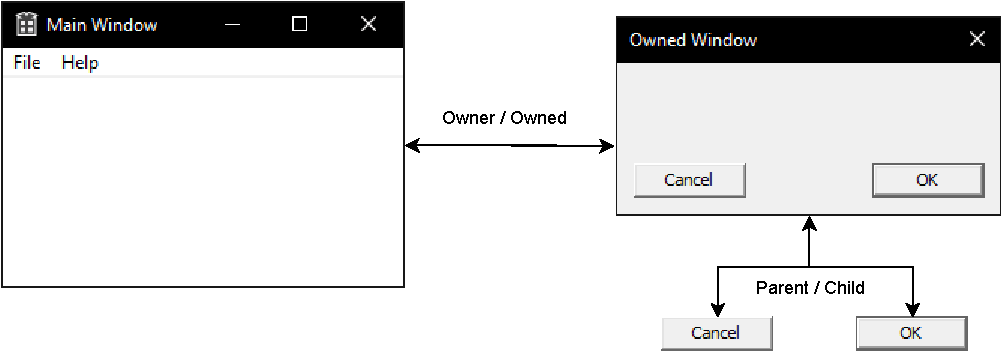
\includegraphics[width=\columnwidth]{obrazky-figures/windows_rels.pdf}
	\caption{Example of owner/owned and parent/child relationships between windows.}
	\label{windowsExample}
\end{figure}

\subsubsection{Object handles}
\label{ch2handle}
In Windows, there is no direct access to system resources like files, threads, windows, or graphic images like icons. These system resources are called objects and are unrelated to the C++ object-oriented implementation of objects. For an application to be able to access an object, it needs to obtain an object \textit{handle}.

A \textit{handle} is an opaque data type to access a system resource via the usage of related Windows API functions, which require an object's handle to identify the said object. The value has no real meaning outside of Windows operating system. One can imagine it as an entry of an internal Windows object table. An application can obtain a handle through various Windows API functions, depending on the object the application is trying to access, i.e., using the \lstinline{CreateFile}\footnote{\url{https://docs.microsoft.com/en-us/windows/win32/api/fileapi/nf-fileapi-createfilew}} function to access a file, which returns a handle on success.\cite{HandlesAndObjects}

Handles are kept and managed internally. Depending on the object, a single object can have either multiple handles or be limited to a single handle at a time with exclusive access.\cite{WinHandleLimits}

\subsubsection{Function results}
For functions, which return handles, it is easy to tell whether or not the function succeeded at its job. Check whether or not the returned handle is invalid. On the other side, a bunch of lower-level Windows API functions returns \textit{NTSTATUS} as a result.

NTSTATUS is a 32-bit unsigned integer value, which is the result error code of an operation, i.e., a Windows API call. This means that, in general, the value of zero means success, and anything above zero is an error code, holding information about what operation failed. This has an exception, where the values \lstinline{0 - 0x3FFFFFFF} define the success status type, and values 
\lstinline{0x40000000 - 0x7FFFFFFF} define an information status type. This is easily checked with the \lstinline{NT_SUCCESS(x)} macro, where \lstinline{x} is NTSTATUS.\cite{WinNTSTATUS}\cite{WinNTSuccess}

\subsubsection{Registry}
The Windows registry is a hierarchical database containing data critical for the Windows operating system's operation, services, and applications that run on it. Data is structure is essentially in a tree format, where the nodes are called \textit{keys}. A key can contain other keys - \textit{subkeys} and entires of data - \textit{values}. 

Registry values have a name, type, and value. Value types are mostly standard Windows types (\ref{winIntegers}) like a double-word, a zero-terminated string, or a generic binary value. There are several predefined (root) keys, each serving a different purpose either for the operating system itself, services, applications, or classes. The root keys are always open and are noted by the \lstinline{HKEY_} prefix.

\begin{figure}[htb!]
	\centering
	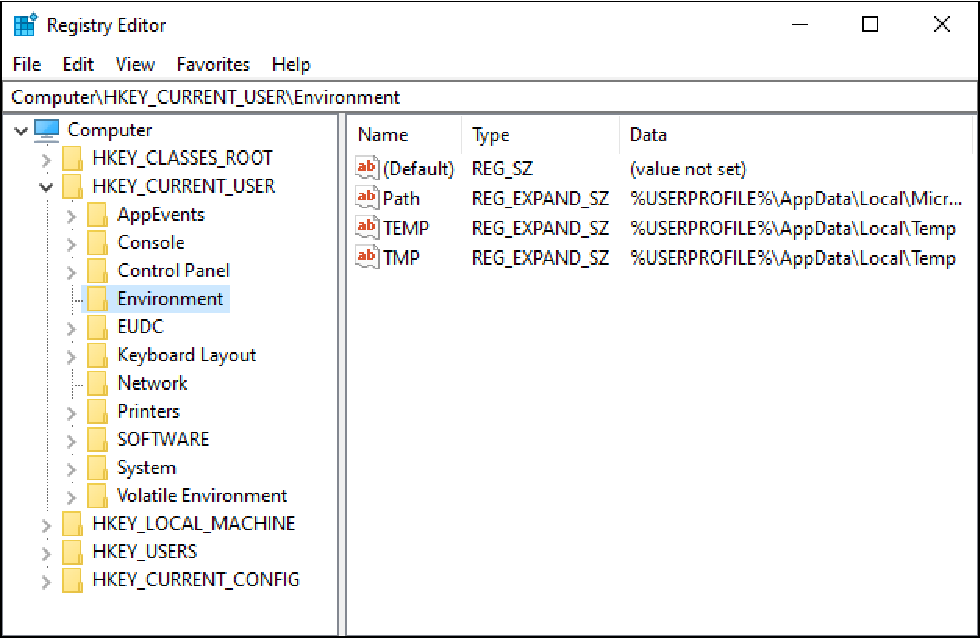
\includegraphics[]{obrazky-figures/regedit.pdf}
	\caption{Browsing Windows registry using the Registry Editor.}
	\label{winRegedit}
\end{figure}

To access a value of a key, one must know its path. The path is a string consisting of all the keys and subkeys, ranging from the root to the leaf key, divided by the backslash character.\cite{WinRegStruct}
For example, in Figure \ref{winRegedit}, to access a value inside the \lstinline{Environment} subkey, the path would be \lstinline{HKEY_CURRENT_USER}\textbackslash{}\lstinline{Environment}. The Windows API provides macros for root key specification, which would allow the programmer to emit the specified root key from the path.

For an application, the registry can save user preferences, various settings, remember selected options, or track the application's usage. It is also useful to make the application run automatically upon startup, as implemented in section \todo{autorun}.

\subsubsection{Thread synchronization}
There are many ways to synchronize threads in Windows. These include, but are not limited to: Events, Semaphores, Mutexes, Interlocked API, and Slim reader/writer locks (SRW locks), listed by \cite{WinSyncFuncs}. As this project makes use of SRW locks, this subsection will explain only those in the following.

As SRW lock is a simplified version of a semaphore, which is according to \cite{WinSemaphores} described as a synchronization object which is useful in controlling a shared resource between multiple threads. A semaphore has a set number of threads that are allowed to access the resource simultaneously. When a thread is done with using the resource, another thread is allowed to use it. As specified by \cite{WinSRW}, an SRW lock takes the thread's intent with the shared resource into account and is optimized for speed and performance. If a thread wants to read a resource, it can lock the resource in a \textit{shared mode}. If a thread wants to write to a resource, it can lock the resource in the \textit{exclusive mode}. If a resource is not locked, it can be locked in either mode. 

The exclusive mode works just like a semaphore with a single allowed thread. The access is always exclusive as no other threads can simultaneously access the resource, even if some threads only want to read the resource.
The shared mode allows for read-only access to the resource by multiple threads if the lock is not locked in exclusive mode.

Neither mode has a priority of acquiring the lock, there is no order or a queue of access, so if two threads want to acqurie an SRW lock, it is not predictable which thread will acquire the lock in different modes. The lock is the size of a pointer, which means faster access but rather limited amount of information stored about the state of the lock. While being simple, it is sufficient enoguh to solve many thread synchronization problems, such as \textit{"The Readers-Writers Problem}\footnote{\url{https://www.u-aizu.ac.jp/~yliu/teaching/os/lec07.html}}.

\subsection{Microsoft Foundation Class Library}
This section introduces the Microsoft Foundation Class Library (MFC) and aims to provide an overview of important designing functions, implementing the user interfaces.

MFC is an object-oriented C++ library, which abstracts and wraps the non-object-oriented Windows API. It is useful for designing and creating user interfaces, small or large dialog boxes, windows, implementing network services, network communication, threading, and more, as described by \cite{MFCDesktop}.

\subsubsection{Relations to Windows API}
As mentioned in previous sections, MFC allows for much easier desktop application development by abstracting and wrapping a lot of the Windows API, originally only written in C, into the object-oriented C++ programming language.

\begin{lstlisting}[caption={Showing a window using Windows API and MFC}, label=showWindowEx]
//Windows API - Using C
HWND hMainWnd = CreateWindowW(...);
ShowWindow(hMainWnd, SW_SHOWNORMAL);

//MFC - Using C++
AfxGetMainWnd()->ShowWindow(SW_SHOWNORMAL);
\end{lstlisting}

Listing \ref{showWindowEx} showcases an example of showing the main window (\ref{ch2Windows}) using both APIs and an instance of abstracting the window handle away in favor of using a window C++ object. Calling the \lstinline{ShowWindow}\footnote{\url{https://docs.microsoft.com/en-us/windows/win32/api/winuser/nf-winuser-showwindow}} function directly from a window object is a lot more straightforward and convenient than handles. However, it is important to keep in mind that MFC still internally uses the Windows API.
This means, if there is a need for a handle of an MFC object, there are supportive functions like \lstinline{GetSafeHwnd}\footnote{\url{https://docs.microsoft.com/en-us/cpp/mfc/reference/cwnd-class?view=msvc-160##getsafehwnd}}, which return the internal object handle.

\subsubsection{Coding conventions}
All global, static MFC functions are marked with an \lstinline{Afx}, prefix (Application Framework Extension). 

\subsubsection{Wrappers}

\subsubsection{Strings}

\subsubsection{Exception handling}

\todo{Overview key MFC parts for this project}

\section{Virtual file systems}
This chapter serves as an overview of available virtual file system technologies that would allow for direct integration with the Windows desktop environment. Such an instance of virtual file system implementation is a Filesystem in userspace (FUSE), "a file system in which an ordinary userspace process provides data and metadata."\cite{FUSE}

This exact implementation does not exist on Windows without a kernel-mode driver\cite{WinKernelFS}. Since creating a kernel-mode driver is out of this thesis's scope, the details of how this can be implemented using a third-party virtual file system software are shown in section \ref{vfsapitypes}.

The following sections contain the introduction to files, file systems, and an overview of available third-party virtual file system software that can be considered a valid option for this project's intent.

\subsection{Introduction to file systems}
The following section helps to understand what a file system is, which operations are the file system's responsibility, how it talks to the file system, how it is defined on a typical file system.

\subsubsection{File}
\label{file}
Generally, in Windows, a \textit{file} is a unit of data in a file system. A file is stored on a storage device\footnote{i.e. Hard Drive} and consists of one or multiple streams of bytes, which hold related data, and a set of attributes that describe the file and its data. The file system manages it, and any application that wants to access, read, write, or execute a file or its attributes has to interact with its respectable file system to do so. A file must follow the file systems' rules, i.e., a file must have a unique name in its directory in NTFS\footnote{New Technology File System}.\cite{FilesAndClusters}

Files in Windows are never accessed directly. Instead, applications on Windows can access a file through its handle (Section \ref{ch2handle}). When a file is opened, a handle is associated with it until the requesting process terminates or the handle is closed. Each handle is unique to each process that opens a file, and depending on which type of access to the file was requested, if one process holds a handle to a file, a second process trying to open a handle to the same file might fail.\cite{FileHandles}

\subsubsection{Filesystem}
A file system is a program that describes how files are stored on a storage device. It allows applications running on the system to access, read and store files. All Windows supported file systems have the following storage components:\cite{LocalFileSystems}

\begin{itemize}
    \item \textbf{Volumes}
    \item \textbf{Directories}
    \item \textbf{Files}
\end{itemize}

A Volume is where the file system resides, is the highest level of organization in a file system, and has at least one partition, a physical disk's logical division.\cite{WinVolumeMgmt} For this project's purposes, only volumes with a single partition (simple volumes) will be considered. Such volume can be called a \textit{drive} if it is recognizable and accessible by its assigned \textit{drive letter}. 
A drive letter is a single capitalized letter of the alphabet ranging from A to Z, meaning Windows only supports a maximum of 26 drives with drive letters at the same time. For simplicity, the process of assigning a volume to a drive letter while making it accessible in the system will be referred to as \textit{mounting} the volume (The system can mount volumes to directories as well).

A directory is a hierarchical collection of files, can itself be organized into a directory, and has no limitations on the number or capacity of files that it contains. The only limit is defined by the file system itself and the capacity of the storage device.\cite{WinDirectoryMgmt} It is important to remember that a directory can be referred to as a file with a special flag \lstinline{FILE_BACKUP_SEMANTICS} inside the Windows API.

A file (\ref{file}) is the related data, and it can be organized into a directory or reside directly in the root of a volume.

\subsubsection{File path formats}
Windows uses the standard, traditional DOS\footnote{Disk Operating System} path format, which consists of the following components:

\begin{itemize}
    \item \textit{A volume or drive letter} - It is expected to be followed by the volume separator character\footnote{The colon character (:)}
    \item \textit{A directory name} - The directory separator character\footnote{The backslash character (\textbackslash{})} separates subdirectories within the hierarchy
    \item \textit{An optional filename} - The directory separator character separates the file path and the filename
\end{itemize}

If all three components are present, the path is called an \textit{absolute} path. If no volume is specified and the path begins with the directory separator character, it is relative to the current drive's root. Otherwise, it is relative to the current directory.\cite{WinPathFormats}

\begin{table}[!hbt]
\centering
\caption{Examples of valid file paths}
\label{filepathsex}
\begin{tabular}{|l|l|l|l|}
\hline
\textbf{Path} & \textbf{Description} \\ \hline
C:\textbackslash{}dir\textbackslash{}test.pdf       & Absolute path from the root of drive \textit{C}    \\ \hline
\textbackslash{}dir\textbackslash{}test.pdf      & Relative path from the root of current drive     \\ \hline
test.pdf       & Relative path from the current directory     \\ \hline
\end{tabular}
\end{table}

\subsection{Virtual Filesystems}
\label{vfs}
A virtual file system is an abstraction of a regular file system - any information, any data, can be organized and presented as a file system. It does not require a storage device to reside on, as it can use one of the existing ones and reside and extend upon it. It can set its own rules on volume, directory, and file management and enforce them. A virtual file system's power also comes from integrating closely with the Windows operating system - hooking into the system's internal file operations and handling them in its own way.

To achieve this, this project uses a third-party virtual file system software, which exposes a virtual file system API. In general, such an API usually allows creating of a virtual file system by providing the programmer with a list of file operation functions that he must implement. These usually consist of functions that handle creating files, deleting files, reading files, etc. Once these functions are implemented, the user-mode library used to implement them provides them to the kernel-mode driver, allowing this new file system to be recognized by Windows. The process of calling implemented file operations works in reverse order. For example, when opening a file, the Windows I/O\footnote{Input\textbackslash{}Output} subsystem runs in kernel mode, forwards this information to the file system driver, invoking user-implemented functions request and handle the file operation (open the file).\cite{GitDokany}

This means that a virtual file system must implement all the Windows operating system's important file operations to be functional. Upon implementation, a file system can even be shown directly in the Windows Explorer and be accessible to all running programs if the virtual drive of the file system is mounted. This is usually done internally within the third-party API. The following subsection covers some of the popular options of virtual file system software.

\subsubsection{Virtual file system software}
\label{vfsapitypes}
In general, there two ways a virtual file system software can implement a virtual file system API:

\begin{itemize}
    \item Native API
    \item FUSE Compatibile API
\end{itemize}

A \textit{Native API} aims to be as close to the intended system it interfaces with as possible, without potentially harmful compromises at the cost of cross-platform compatibility or other factors unrelated to the system. This type can potentially be lower-level than FUSE API and must be well documented by its provider to be usable. As noted by its name, tying closely to a single system means the API focuses on working on the intended system as seamlessly as possible. For windows specifically, native API requires two components, a kernel-mode driver and a user-mode library which interacts with it.

\begin{itemize}
    \item \textit{Pros}: Good optimization, coding constructs similar to the targeted system, all features of the targeted system
    \item \textit{Cons}: Little to no cross-platform compatibility, lower-level API requires deeper knowledge of the targeted system, a steeper learning curve
\end{itemize}

The \textit{FUSE Compatible API} is meant to be compatible with FUSE, a high-level API originally only for Linux. Compatibility with FUSE allows for cross-platform compatibility with little to no changes to the virtual file system's implementation. For Windows specifically, the implementation of file systems is vastly different from Linux. The usage of a FUSE compatible API comes with its compromises, such as lower performance, or excluding some of the features only present in Windows, i.e., volume labels.\cite{WinFspVSFUSE}\cite{FUSE}

\begin{itemize}
    \item \textit{Pros}: Cross-platform compatibility, easier development with higher-level API, well-documented API
    \item \textit{Cons}: Lack of Windows-specific features, restricted by POSIX standards
\end{itemize}

For this thesis, it is much preferable to choose an API software option that includes a native API, as cross-platform compatibility is not a requirement. Thus, there is no need for any restrictions. Additionally, being able to use Windows-specific file system-related features is a step towards a better user experience. An open-source license of the software would also be preferred.

\subsubsection{Dokany}
Dokany is one of the oldest yet still fully functional pieces of virtual file system software. It was created in 2007, and while undergoing a switching of its developers, it is still being developed today.

\begin{itemize}
    \item \textit{Supported API types}: Native, FUSE wrapper
    \item \textit{Supported languages}: C (default), Java, Delphi, DotNet, Ruby
    \item \textit{Supported architectures}: x86, x64, ARM, ARM64
    \item \textit{Supported desktop operating systems}: Windows 7 SP1 / 8 / 8.1 / 10
    \item \textit{Open-source}: Yes
    \item \textit{Provides a driver}: Yes
\end{itemize}

In conclusion, Dokany is a well-supported, stable piece of software, nearly an ideal choice for projects that pay excessive attention to software stability and compatibility while creating a file system in various, even higher-level programming languages, rather than just the low-level C.\cite{GitDokany}\cite{DokanDevIo}

\subsubsection{VFSForGit}
Virtual File System for Git is software developed by Microsoft to enable Git\footnote{\url{https://git-scm.com/}} at a high level, enterprise scale. VFSForGit virtualizes a Git repository into a virtual file system. This is a form of integrating the files, which are not physically present on the user's computer, rather still being present on the Git repository while being displayed. The user can download the contents of the files on request via the application's user interface. 

\begin{itemize}
    \item \textit{Supported API types}: Native GVFS Protocol\footnote{\url{https://github.com/microsoft/VFSForGit/blob/master/Protocol.md}}
    \item \textit{Supported languages}: Git commands
    \item \textit{Supported architectures}: x64
    \item \textit{Supported desktop operating systems}: Windows 10 version 1607, or later
    \item \textit{Open-source}: Yes
    \item \textit{Provides a driver}: Yes
\end{itemize}

VFSForGit is a virtual file system software aimed towards usage with Git repositories, especially at larger scales. It doesn't provide many languages or options for architectures and only supports newer versions of Windows 10. With those restrictions in mind, it is still being supported and is a useful tool for accessing Git repositories in the Windows environment.\cite{GitVfsForGit}\cite{VfsForGitMS}

\subsubsection{WinFsp}
Windows File System Proxy is a performant, stable collection of software components, which allows for implementing a virtual file system using one of its supported API layers. The focus of WinFsp is on high compatibility with NTFS, the default file system of Windows. This allows for smooth integration with the Windows environment and virtual file systems, which use or extend NTFS.

\begin{itemize}
    \item \textit{Supported API types}: Native, FUSE compatibility layer
    \item \textit{Supported languages}: C, C++, DotNet
    \item \textit{Supported architectures}: x86, x64, ARM, ARM64
    \item \textit{Supported desktop operating systems}: Windows 7 and above
    \item \textit{Open-source}: Yes
    \item \textit{Provides a driver}: Yes
\end{itemize}

WinFsp is a great option for any virtual file system implementation, running only on Windows. Whether it is one of the older versions of the operating system, or the newer one, WinFsp provides continuous support and compatibility with those systems while keeping the officially supported languages of its API layers both lower and higher level, thanks to the inclusion of C++ and DotNet. It is a great choice for any project starting from scratch.\cite{GitWinFsp}

\subsubsection{Conclusion}
The third-party file system software of choice for this project is Windows File System Proxy (WinFsp). VFSforGit could not be used because of its limitations and focus on Git repositories since the VDU project does not expose any Git repositories. This is further mentioned during analysis in chapter \ref{ch_analysis}. Dokany was a great option, stable, supported, and similar with compatibility layers to WinFsp. On the other hand, WinFsp has native API support for C++, which allows for cleaner and easier to understand code, and offers much better performance and optimization than Dokany. Various file system operation tests that compare versions of WinFsp against Dokany and NTFS prove this. These charts are displayed in figures \ref{winfsp_file_tests} and \ref{winfsp_rdwr_tests}.

\begin{figure}[htb]
	\centering
	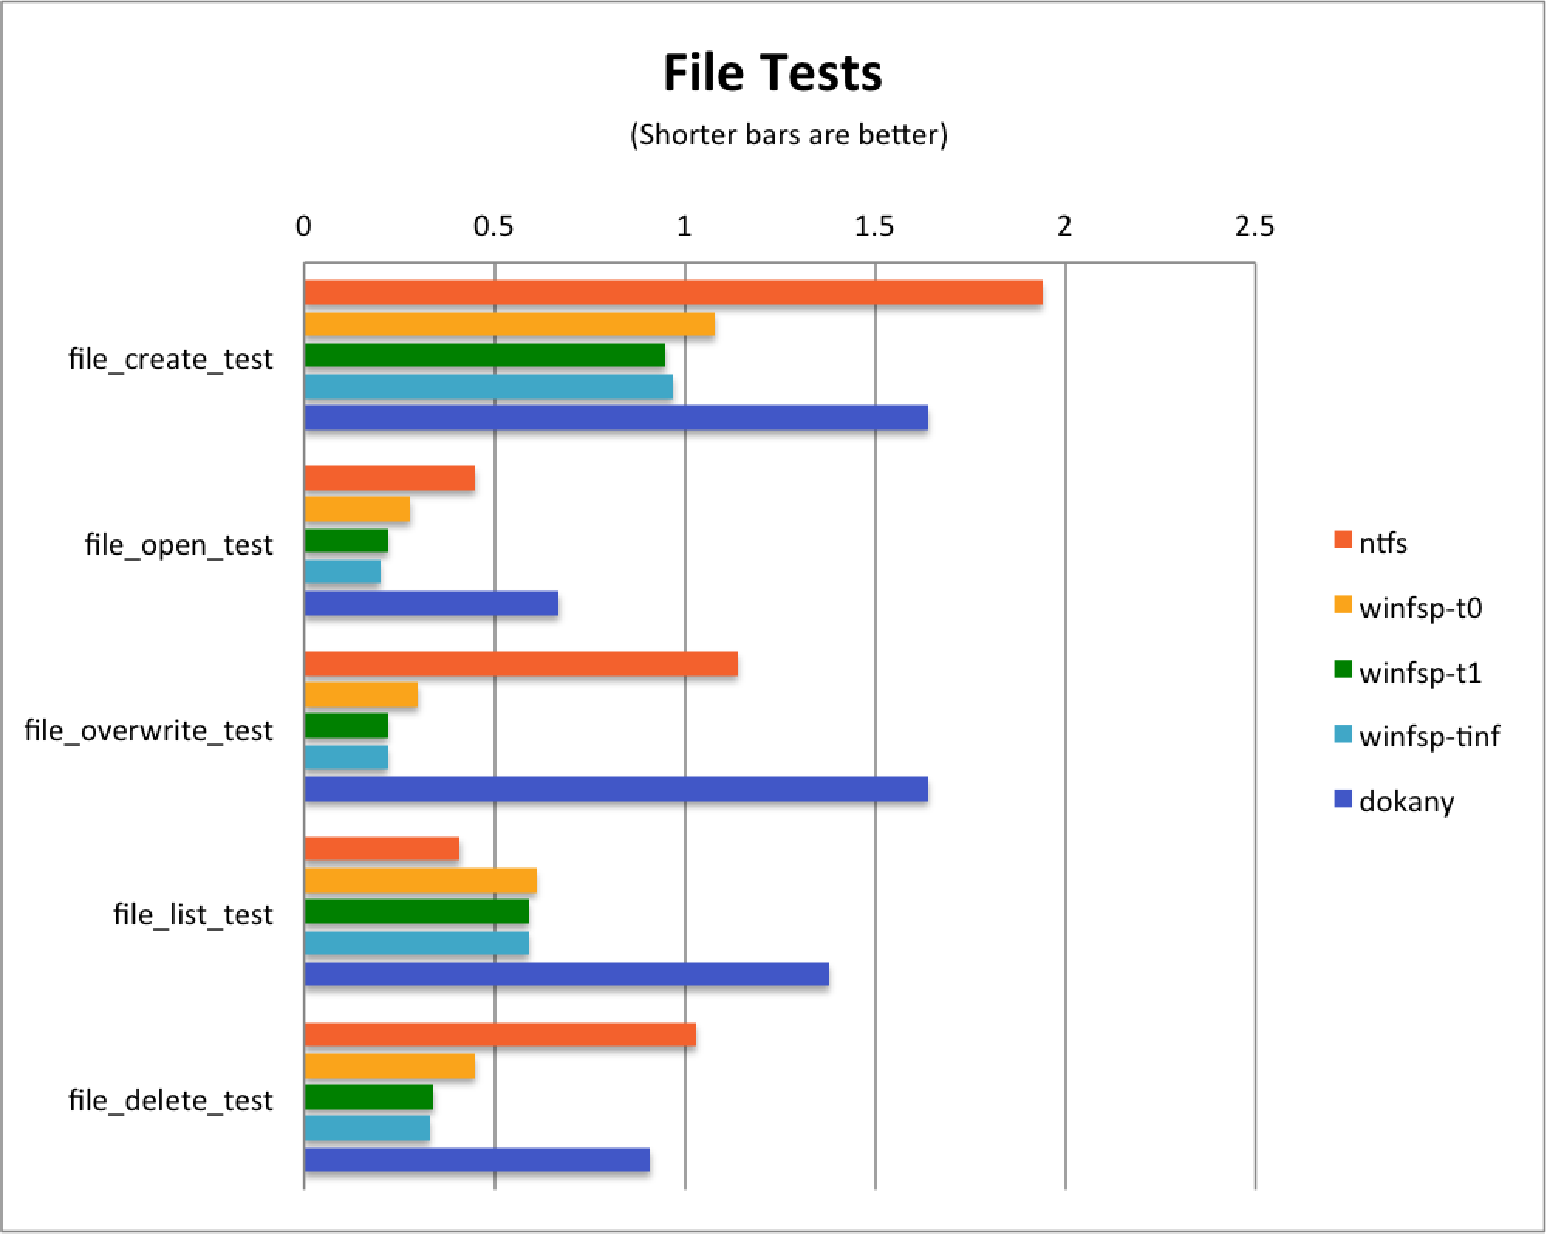
\includegraphics[width=\columnwidth]{obrazky-figures/file_tests.pdf}
	\caption{File comparison tests of WinFsp and Dokany. Source:\cite{GitWinFsp}}
	\label{winfsp_file_tests}
\end{figure}

\begin{figure}[htb]
	\centering
	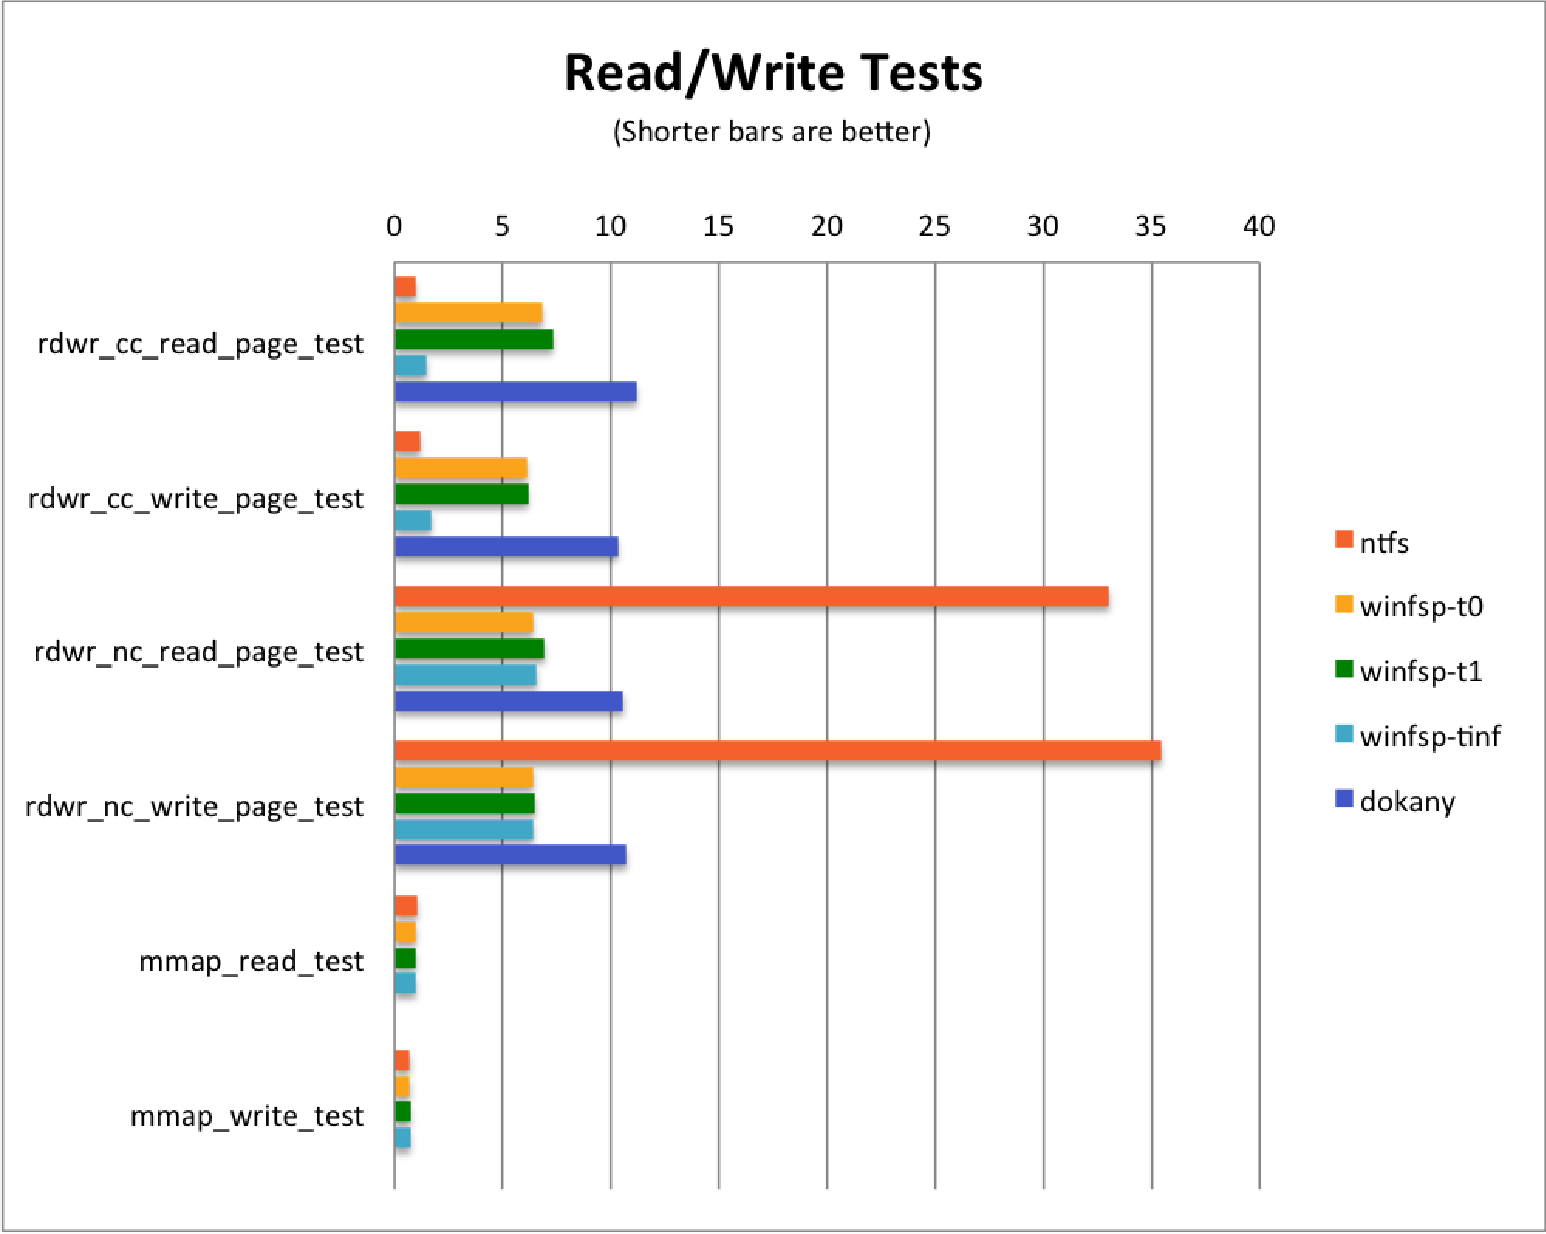
\includegraphics[width=\columnwidth]{obrazky-figures/rdwr_tests.pdf}
	\caption{Read and write comparison tests of WinFsp and Dokany. Source:\cite{GitWinFsp}}
	\label{winfsp_rdwr_tests}
\end{figure}

\section{Additional technologies}
This section provides an overview of additional technologies used in this thesis, which do not fall under any specific category. It includes the Hypertext Transfer Protocol (HTTP), the Representational State Transfer (REST) and how it makes use of HTTP, along with a formal description format OpenAPI, used during the analysis in Chapter \ref{ch_analysis}. 

\subsection{Hypertext Transfer Protocol}
The Hypertext Transfer Protocol, as described by \cite{MozillaHTTP}, is a simple, stateless communication protocol used for fetching resources. A resource can be anything that can be named, ranging from images, documents to generic files. HTTP is designed as a client-server type of protocol, in which a client and a server exchange information using HTTP messages. An HTTP message can be one of two types:
\begin{itemize}
    \item \textit{HTTP Request} - From client to server
    \item \textit{HTTP Response} - From server to client
\end{itemize}
\subsubsection{HTTP request}
An HTTP request consists of the following elements, in order:
\begin{enumerate}
    \item \textit{Method} - Defines the requested operation with the resource
    \item \textit{Path} - Location of the resource
    \item \textit{Protocol version} - Version of HTTP
    \item \textit{Request headers} - Additional information about the resource
    \item \textit{Content} - Contains the content of the resource sent to the server
\end{enumerate}
\subsubsection{HTTP response}
An HTTP response consists of the following elements, in order:
\begin{enumerate}
    \item \textit{Protocol version} - Version of HTTP
    \item \textit{Status code} - Defines the requested operation with the resource
    \item \textit{Status message} - Location of the resource
    \item \textit{Protocol version} - Version of HTTP
    \item \textit{Response headers} - Additional information about the resource
    \item \textit{Content} - Contains the content of the resource sent to the client
    \end{enumerate}
\subsection{Representational State Transfer}
According to \cite{RestAPI}, The Representational State Transfer represents an architectural style of developing RESTful web services, which allows the developer to take advantage of an already existing protocol. In the case of web services, this protocol is HTTP. REST conforms at the very least to the most basic REST constraints, as defined by its creator \textit{Roy Thomas Fielding}:

\begin{itemize}
    \item \textit{Client-Server} - Separates the client's side and the server's side
    \item \textit{Stateless} - Each request must contain all necessary information necessary to understand the request
    \item \textit{Cache} - Requests must be labeled as cacheable or non-cacheable. Improves network efficiency if it is available
\end{itemize}
\subsubsection{REST using HTTP}
The key abstraction of information in REST is a \textit{resource}. This definition is similar to the HTTP resource -  a resource can be anything that can be named and might be a potential target of a request, e.g., a document, an image, a data file. The REST \textit{endpoint} refers to the \textit{path} of an HTTP request. The content of a resource is usually transferred as the \textit{content} of an HTTP message. HTTP headers are useful for storing additional information about a resource, such as the file name, size of the content, encoding, etc. The HTTP method specifies the operation with a resource, which should conform to the REST API documentation of the server. An example of a simple REST API description is listed in Table \ref{restapiex}.
\begin{table}[hbt]
\centering
\label{restapiex}
\begin{tabular}{|l|l|l|l|}
\hline
\textbf{Method} & \textbf{Endpoint} & \textbf{Description} \\ \hline
 GET & /users & Get all users \\ \hline
 POST & /users/john & Update an user  \\ \hline
 DELETE & /users/john &  Delete an user \\ \hline
 PUT & /users & Add an user \\ \hline
\end{tabular}
\caption{An example of a table of REST API endpoints }
\end{table} 

\subsection{OpenAPI}
The OpenAPI Specification is a description format for REST APIs. This format is handy for creating more formal descriptions of the entire API can be described with just a single file written in the OpenAPI format, which supports file formats of either YAML\footnote{A recursive acronym for "YAML Ain't Markup Language"} or JSON\footnote{JavaScript Object Notation}. According to \cite{SwaggerDocs}, the OpenAPI format is capable of describing:

\begin{itemize}
    \item Available endpoints and operations on each endpoint
    \item Operation parameters, and input/output for each operation
    \item Authentication methods
    \item Contact information, terms of use, other information
\end{itemize}

As Listing \ref{openapiex} shows, the OpenAPI format is easily readable and understandable for both machines and humans. Additionally, many third or first-party services provide a way to visualize the API in a graphical, user-friendly format, i.e., the Swagger Editor\footnote{\url{https://editor.swagger.io/}}. An example of a rendered graphical representation of the VDU server's REST API is displayed in Figure \ref{swagger_result}.
\begin{lstlisting}[caption={An example of an OpenAPI file in the YAML format}, label=openapiex]
#A simple documentation of a /ping endpoint
openapi: 3.0.0 
info:
  version: '1.0' 
  title: An amazing API
  description: A formal description
servers: #Server URL for testing
  - url: 'https://localhost:4443'
paths: #Endpoint descriptions
  /ping: #Endpoint path
    get: #Method
      parameters: [] #Call parameters
      description: To test a connection.
      responses: #Possible responses
        '204':
          description: Ping success!
\end{lstlisting}
%=============================================================================================================================
\chapter{Specification}
\label{ch_specification}
The goal of this thesis was to design, implement and test a client side application for Windows operating system, which integrates with the Windows desktop environment. This application should be able to connect to the VDU server and secure access to remote files present on the server, as they are being accessed by the user. The specification was provided by multiple sources:
\begin{itemize}
    \item \textit{Thesis specification} - Provided the exact steps this thesis should be taking
    \item \textit{VDU API documentation} - Provided a detailed, non-formal description of the VDU server's API
    \item \textit{Consultations with supervisor} - Provided more details, helped to narrow down design choices and testing ideas
\end{itemize}

%=============================================================================================================================
\chapter{Analysis}
\label{ch_analysis}
%=============================================================================================================================
This chapter will tackle the first step of creating an application, the analysis, and steps taken during an analysis of provided documentation of the VDU server. It will introduce required technologies to understand and handle them. Results of the analysis are present at the end of this chapter.

\todo{Include google docs pdf of requirements?}

\section{Formalization}
Considering the provided documentation, formalization means creating an OpenAPI specification based on the documentation's plain text version. A formalized specification allows for better readability, understanding, development, and testing on the developer's side. The formalized specification's concrete usage is covered in chapter \ref{ch_implementation}, implementing the client, and \ref{ch_testing} for implementing and testing a mock server.

\subsection{Creating the specification}
Formalizing the provided documentation consists of reading and understanding all the API endpoints and their access or usage restrictions and manually creating an entry for each in an OpenAPI file. Each entry has its own possible status codes, headers, and content, which endpoint could return. For this project, I used the Swagger Editor, which allowed me to document the VDU API more comfortably. The editor's great advantage is that it can render the OpenAPI specification file in an HTML\footnote{Hyper-Text Markup Language} 5 format, as shown in Figure \ref{swagger_result}.

\begin{figure}[htb]
	\centering
	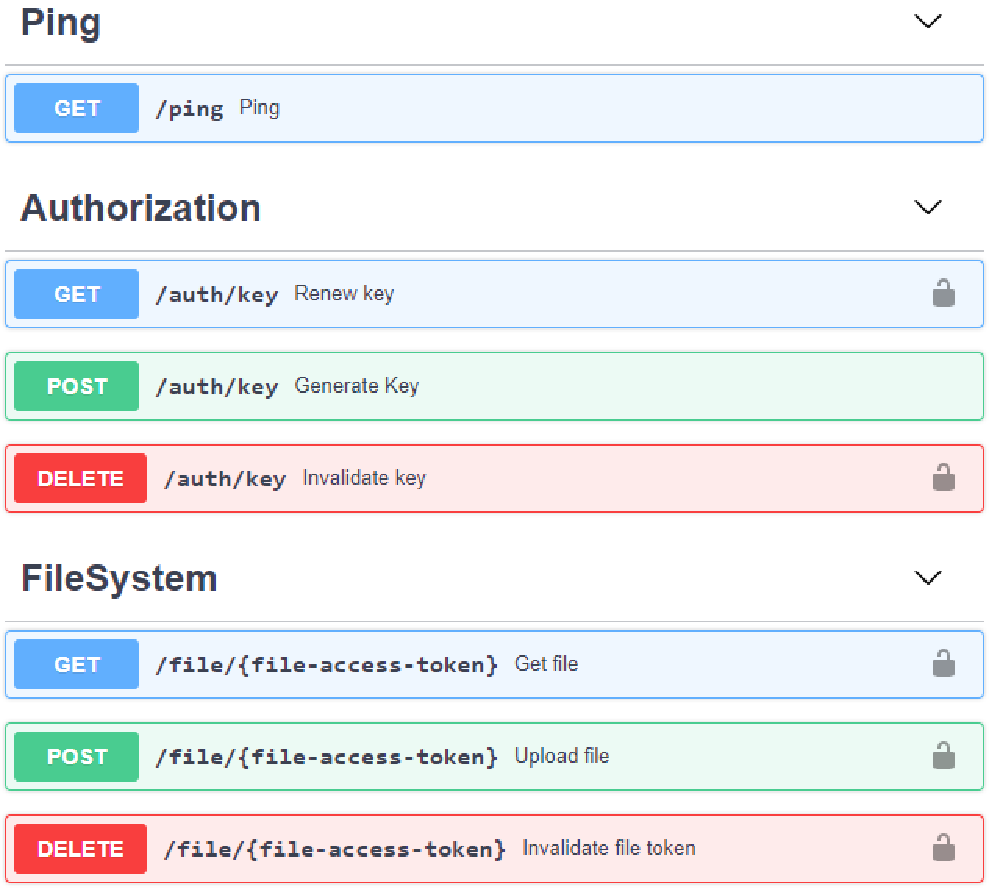
\includegraphics[width=\columnwidth]{obrazky-figures/swagger_result.pdf}
	\caption{VDU REST OpenAPI 3.0 summary, rendered using the Swagger Editor, authentication requirement is signified by the lock icon.}
	\label{swagger_result}
\end{figure}

I analyzed and noted all the API access requirements, each method, its parameters, return values, and how they tie to each other from the formal, well-specified API documentation. Afterward, I discussed this information further with my supervisor, which allowed me to understand better how the API works and how it should interact.

\section{Results}
\label{analysis_results}
This section will summarize the result of the VDU API documentation analysis. These results are used to guide the design of the application in Chapter \ref{ch_design}.

\subsection{Endpoints}
This subsection lists all available VDU API endpoints, as shown in Figure \ref{swagger_result}, and provides an overview of their usages. Some endpoints require an \textit{X-Api-Key} (API key) for successful access.

\begin{itemize}
    \item \textit{GET} \textit{/ping} - Tests a connection to the server
    \item \textit{POST} \textit{/auth/key} - Authenticates an user by name or email. Client secret can be included in the content if necessary. Returns API key on success.
    \item \textit{GET} \textit{/auth/key} - Returns a new API key with new expiration time, refreshes session
    \item \textit{DELETE} \textit{/auth/key} - Invalidates API key
    \item \textit{GET} \textit{/file/\{file-access-token\}} - Returns file contents, additional file information is in the response headers
    \item \textit{POST} \textit{/file/\{file-access-token\}} - Uploads file contents, additional file information has to be in the request headers
    \item \textit{DELETE} \textit{/file/\{file-access-token\}} - Invalidates a file token, does NOT delete the file from VDU system
\end{itemize}

\subsection{Access}
Both client and server must use a secure TLS\footnote{Transport Layer Security} channel to access the VDU API, while the server must have a valid server-side TLS certificate. This implies the usage of HTTPS protocol to access the API. The client-side certificate is optional and allows the user to omit the client secret from the authentication endpoint.

The authentication is done using an API key obtained from the \lstinline{POST /auth/key} endpoint. An API key has its expiration date, which a client must respect, and the key has to be refreshed using the \lstinline{GET /auth/key} endpoint if it is about to expire. The client can prematurely invalidate the API key with the \lstinline{DELETE /auth/key} endpoint.

File tokens, seen as the path parameter \textit{\{file-access-token\}} in the \lstinline{/file/} endpoint, are generated from the proprietary VDU web user interface. Each token represents a single file, has an expiration date, and can be prematurely invalidated using the \lstinline{DELETE /file/} endpoint. This file can be modified using the \lstinline{POST /file/} endpoint, which includes modifying its content and file name. A file can be read-only, meaning that the server will deny any modification request.

\subsection{Version control}
The file version control system is handled on the VDU server. The VDU client does not manage or control the version of a file. This version is noted as an \lstinline{ETag} header, which can be any string. The VDU server can change this tag upon successful file upload on the server's side, which could lead to invalidation of the user's file token directly after the upload. The client has to adapt to the server-side version, which it receives via a response from the \lstinline{/file/} endpoint, and must not propose its own.


%=============================================================================================================================
\chapter{Design}
\label{ch_design}
%=============================================================================================================================
This chapter aims to design the application based on knowledge from previous chapters. The designing process consists of two main parts - the visual and the inner application design part. The visual part takes care of the user interface, user experience, all the windows, menus, buttons, and overall feeling of the application for the user. The inner application part revolves around the class structure and relationships, chooses coding practices and various internal options for designing the application, which is implemented in chapter \ref{ch_implementation}.

\section{User interface}
The user interface includes all the application's visual elements and all the other elements a user can interact with while using the application. Based on the VDU API documentation analysis of requirements, I listed all important actions and ways users could interact with the VDU client. These key functionalities can be referred to as \textit{user actions}: 

\begin{itemize}
    \item Test a connection to the server
    \item Login/out of the system
    \item Change the virtual drive letter
    \item Input a file token to access a file
    \item Read and modify accessed files, concerning version control
    \item Invalidate a file token of a file
\end{itemize}

The following subsections explain how the application's user interface was thought out, designed, and my thoughts behind those decisions.

\subsection{Integration into Windows environment}

Note that not all of these actions have to be included in the application's user interface. For example, the user can read and modify files via some other application present on the system, completely unrelated to the VDU client. This fact has led me to an important realization. Windows Explorer, a built-in tool for browsing files in Windows, has an amazing user interface that can display files provided by a file system - such as a virtual file system of the VDU client, as displayed in Figure \ref{explorervdudisk}. 
Using Windows File Explorer to provide the functionality of file access-related actions is an intuitive way of integrating with the Windows desktop environment.

There is one more action that the Windows File Explorer is capable of - deleting files. Note that the VDU API does not provide an endpoint for file deletion per se. Rather, an endpoint for invalidating a file token. This means, deleting files downloaded from the VDU server in the virtual file system becomes confusing to use for the user as a file would be deleted only locally, and this action would not invalidate the token. This has led me to an unusual design decision. Re-purposing the file deletion feature to invalidate the file's token and only delete the local file if the server allows so. Thus, the number of action which the VDU client has to implement in its own user interface is reduced even more. 

In conclusion, by using built-in features of existing applications in the Windows environment, specifically the Windows File Explorer, I was able to simplify the VDU client's user interface while keeping its functionality unchanged. Details on how exactly this is implemented and why it is not limited to Windows File Explorer only are explained in chapter \ref{ch_implementation}.

\begin{figure}[htb]
    \centering
    
\includegraphics[]{obrazky-figures/explorervdudisk.pdf}
	\caption{The VDU Virtual Disk as shown in the Windows Explorer.}
	\label{explorervdudisk}
\end{figure}

\subsection{Dialog design}
\label{dialogdesign}
After narrowing down all user actions, as shown in the use case diagram in Figure \ref{usecasediagr}, the next step is to design the actual VDU client interface.

\begin{figure}[htb]
    \centering
    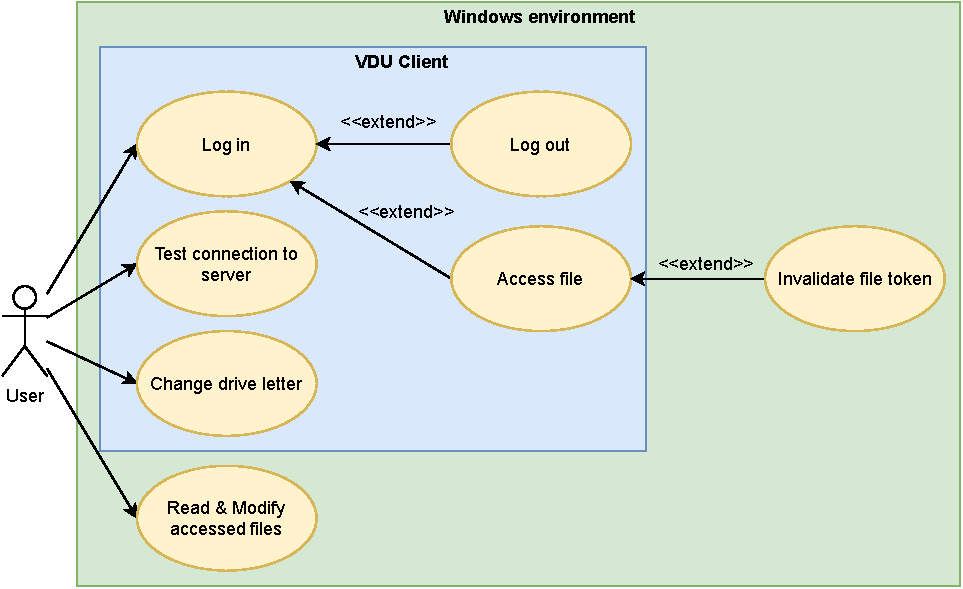
\includegraphics[width=\columnwidth]{obrazky-figures/usecasediagr.pdf}
	\caption{Use case diagram from the view point of an user of the VDU Client system and the Windows environment it resides in.}
	\label{usecasediagr}
\end{figure}

 Considering the low amount of functionality required, I decided to design a simple \textit{Extended Dialog Window} (dialog). The dialog, seen in Figure \ref{clientui}, is separated into three sections:
 \begin{itemize}
     \item \textit{Connection} - Client-Server functionality
     \item \textit{File System} - Local virtual file system functionality
     \item \textit{Status} - Information about the state of the application
 \end{itemize}
The idea behind division was to improve visual clarity while keeping the interface compact and easy to navigate.

\begin{figure}[htb]
    \centering
    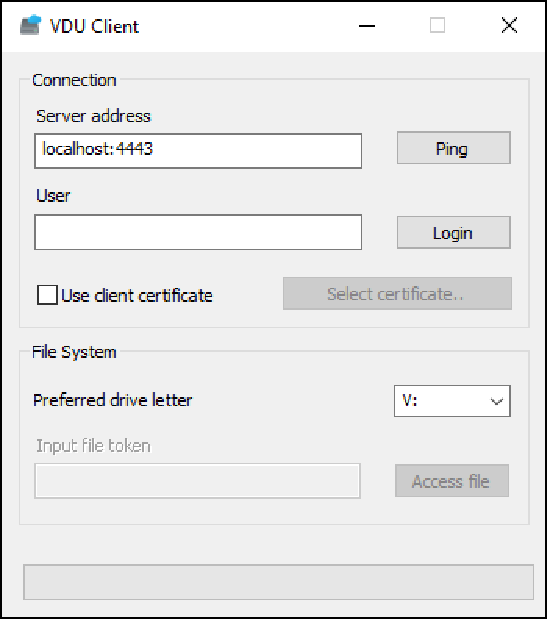
\includegraphics[]{obrazky-figures/clientui.pdf}
	\caption{User interface of the VDU Client application.}
	\label{clientui}
\end{figure}

\subsubsection{Connection section}
This section contains information about the server address, user name, and, if required, a path to a client certificate (client secret) to include the login information. Connection to the server can be tested using the \textit{Ping} button. The \textit{Login} button allows the user to authenticate himself to the server and changes to a \textit{Logout} button upon successfully logging in. Logging in enables all authentication restricted functionality in the following sections and the entire application.

\subsubsection{File system section}
The \textit{Access file} button attempts to download and launch a file from the VDU server, given a token from the input field. The user is also given an option to choose a preferred drive letter for the virtual drive, which the VDU virtual file system will control.

\subsubsection{Status section}
\label{statussectionui}
Containing only a progress bar and a status text, this section informs the user about the application's state. This information includes download progress - visible on the progress bar, connection status, number of accessed files, and currently logged-in user.

\subsection{Dialog tray}
When the VDU application is running, implicitly, so is the dialog window. This is true even if a user is not using the dialog window actively. In a simple use case scenario, the dialog window is only required to log in and access a file. Afterward, it theoretically does not have to be cluttering so much space on the screen and the taskbar. 

This inspired me to design a beneficial addition to the dialog - a tray icon. This icon resides in the tray area of the Windows user interface. The idea is simple, upon closing or minimizing the dialog, the application would stay running in the background, signified by the icon being present. The user can restore the dialog window by simply clicking on the VDU Client icon, displayed in Figure \ref{iconscloud}, in the tray area.

\begin{figure}[htb]
    \centering
	
\includegraphics[width=50px]{obrazky-figures/cloudicon.pdf}
	\caption{Cloud Storage Icon, used as the main icon for VDU client application, Source:\cite{Icons8Cloud}.}
	\label{iconscloud}
\end{figure}

Furthermore, removing the ability to close and exit the application from the dialog window has moved this responsibility to the tray icon. I designed a simple tray menu to fix this problem, depicted in Figure \ref{traymenuex}, which becomes active after right-clicking the icon. The \textit{Exit} option in this menu, shown in the listing, is how the user is supposed to quit using the application.

\begin{figure}[htb]
    \centering
	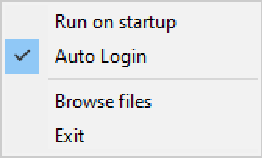
\includegraphics[]{obrazky-figures/traymenu.pdf}
	\caption{Tray menu of the VDU Client application.}
	\label{traymenuex}
\end{figure}

Windows allows applications that put icons in the tray area to display a small text message while hovering the icon - a \textit{tray tip}. I utilized this tray tip to display a compact, text version of the data from the status section \ref{statussectionui} of the dialog, as displayed in Figure \ref{traytipex}.

\begin{figure}[htb]
    \centering
	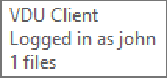
\includegraphics[]{obrazky-figures/traytip.pdf}
	\caption{Example of a tray tip, displaying the state of the application.}
	\label{traytipex}
\end{figure}

\subsection{Responsiveness and notifications}
A good application needs to be responsive and notify the user about important events. Every action directly taken by the user should have a visual response. Given the specifications, the VDU client application will communicate with a server over a network connection. Whether the server resides in a local network or on the internet, it is safe to assume that the application will not finish an action instantaneously. This means a good, responsive application needs to notify the user via the user interface using two types of responses:
\begin{itemize}
    \item \textit{Instant} - Direct visual response to an action, proving to the user that the application is working on the user's request
    \item \textit{Delayed} - A second, more detailed response, once enough information is gathered from the server
\end{itemize}

The application must keep being responsive while handling responses to all actions. How this is implemented is explained in section \todo{Implementation}.

For the VDU client dialog window, an instant response consists of enabling or disabling the related child windows\footnote{e.g. buttons, check-boxes, combo-boxes}. For example, an instant response to clicking the \textit{Ping} button, as displayed on the user interface in Figure \ref{clientui}, would disable the button, making it non-clickable. This button would be then enabled once again along with the follow-up - delayed response.
The delayed response consists of either creating a message box or displaying a Windows notification.

\subsubsection{Message box}
A message box in the VDU client is a simple window, often created as an \textit{owned window} relative to the main window. It is used as either an instant or a delayed response to important actions caused directly by the user, i.e., trying to test a connection to an incorrect server will result in a message box depicted in Figure \ref{messageboxex}. 

\begin{figure}[htb]
    \centering
	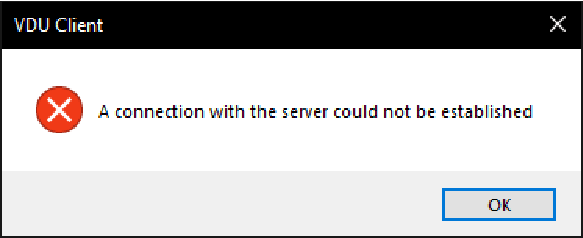
\includegraphics[]{obrazky-figures/messageboxex.pdf}
	\caption{A message box window, displayed after the application fails to connect to a server.}
	\label{messageboxex}
\end{figure}

\subsubsection{Windows notifications}
For less important and rather informative actions, a Windows notification shows up as a response. Such a notification, displayed in Figure \ref{notificationex}, appears, for example, after a successful download of a newly accessed file, along with an automatic startup of the assigned application to the file type. This lets the user know it was the VDU client which caused the application to open.
\begin{figure}[htb]
    \centering
	
\includegraphics[]{obrazky-figures/notificationex.pdf}
	\caption{A windows notification, displayed after a successfully obtaining access to a file in the bottom right corner of the screen.}
	\label{notificationex}
\end{figure}

\section{Class structure}
Choosing the right design of the VDU client's internal components is key to creating a good, reliable, and scalable application. As depicted in the Unified Modeling Language (UML) class diagram in Figure \ref{vduclassdiagram}, the concrete class structure and design's inspiration was the \textit{Single Responsibility Principle} (SRP).

According to \cite{CleanCodeBook}, SRP is a useful design principle to keep in mind while designing object-oriented classes or modules. This is especially useful for applications, which aim to be reliable, easy to maintain, and scalable. SRP states, for example, that a single class should only have a \textit{single reason to change}. This shifts all the responsibilities related to its purpose and allows it to be developed independently from others. Following SRP is a good way to keep software and its code clean and easy to understand. This has led me to design the following classes for the application:
\begin{itemize}
    \item \textit{VDUClient} - Main class of the application
    \item \textit{CVDUClientDlg} - Instantiates and handles the dialog window
    \item \textit{CVDUConnection} - Provides a communication layer with the server
    \item \textit{CVDUSession} - Provides a session functionality for authentication purposes
    \item \textit{CVDUFile} - Represents the structure and data of an accessed file from the VDU server
    \item \textit{CVDUFileSystem} - Implements the virtual file system
    \item \textit{CVDUFileSystemService} - Provides functionality to interact with the virtual file system
\end{itemize}
\begin{figure}[htb]
    \centering
	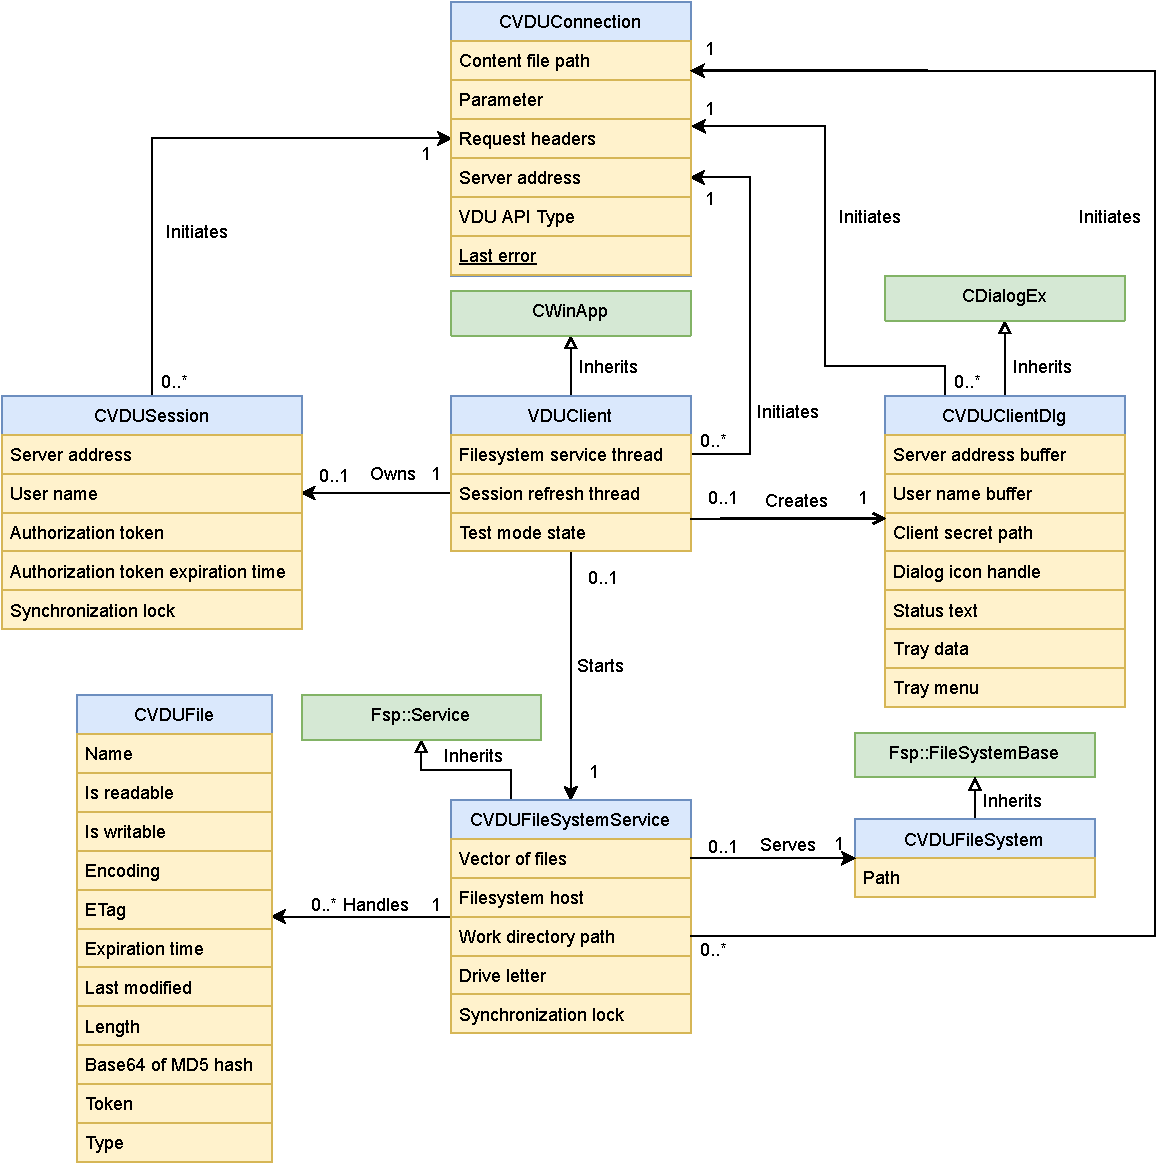
\includegraphics[width=\columnwidth]{obrazky-figures/vduclassdiagram.pdf}
	\caption{UML class diagram of the VDU Client application. \todo{REDO IN THE PROGRAM}}
	\label{vduclassdiagram}
\end{figure}
Each class has a name that implies its purpose and responsibility. All classes rely on each other to exist and can be instantiated for the VDU client to function, except the dialog handling class, \lstinline{CVDUClientDlg}, which is not required to be instantiated when the application's \textit{testing mode} is enabled. The testing mode is used while performing automatic tests on the application in chapter \ref{ch_testing}.

\section{Data storage}
There are many ways to go about storing data for an application. For the VDU client, there are two types of data, which need to be stored:
\begin{itemize}
    \item \textit{Files} - The actual downloaded files from the VDU server, stored using the host file system
    \item \textit{Settings} - The configuration of the application, stored using Windows registry
\end{itemize}

\subsection{Host file system}
For files, it is highly advantageous to store them using the host file system over all other options available. The VDU client stores downloaded files in a temporary folder on the main drive, using the host file system. This folder exists per user, meaning each local user of Windows has their own temporary folder tied to their Windows account. This prevents unintended file sharing if multiple users are using the application on the same system. This folder is emptied each time the application starts and has a randomly generated name upon each creation. All unsaved files will stay in this folder if the system crashes, available for potential data recovery. \todo{Detailed temp?}

\subsubsection{Motivation}
Creating a virtual file system gives freedom to portray any data as files. This fact has inspired me to attempt to store the files using just the systems Random-Access Memory (RAM) of the application. While the speed and accessibility of RAM might make this idea seem plausible, in reality, it would not work well enough for a couple of reasons:
\begin{itemize}
    \item \textit{Space limitations} - Large files might not have enough space
    \item \textit{Inactive RAM usage} - Files not actively in use might prevent other applications from using that space
    \item \textit{No file recovery} - If the system crashes, there is no way to recover unsaved work with the files
\end{itemize}

\subsection{Windows registry}
The application's configuration does not require much space, and as such, the idea of using a custom database or storing it as a file on the host file system seems quite far-fetched. 
One can simplify an application's configuration settings into a simple pair \lstinline{key:value}, where the \textit{key} is a unique identifier of data type \textit{string}, and \textit{value} can be any supported data type on the system. The Windows registry allows applications to store information in this exact format, making it an ideal choice of data storage for the VDU client's configuration settings. Table \ref{vduregistrytable} lists out the concrete settings stored inside the registry by the application.
\begin{table}[hbt]
\centering
\label{vduregistrytable}
\begin{tabular}{|l|l|l|l|}
\hline
\textbf{Name} & \textbf{Data type} & \textbf{Description} \\ \hline
 AutoLogin & double-word & AutoLogin feature state \\ \hline
 ClientCertPath & string & Path to client secret file \\ \hline
 LastServerAddress & string & Last entered server address \\ \hline
 LastUserName & string & Last entered user name \\ \hline
 PreferredDriveLetter & string & Selected preferred drive letter \\ \hline
 UseCertToLogin & double-word & Whether or not to use client secret \\ \hline
 WorkDir & string & Current directory used to store VDU files  \\ \hline
\end{tabular}
\caption{The concrete settings stored by VDU Client using the Windows registry.}
\end{table} 



%=============================================================================================================================
\chapter{Implementation}
\label{ch_implementation}
%=============================================================================================================================
This chapter covers the exact internal implementation of key elements of the VDU client, as described in previous Chapter \ref{ch_design}, which covered the application's overall design. The entire implementation of the application was done using Visual Studio Community 2019, an IDE\footnote{Integrated Development Environment} which is further described in section \ref{ch2vs19}. This chapter makes implicit use of the following macros:
\begin{itemize}
    \item \textit{WND} - Main window object (\lstinline{CVDUClientDlg})
    \item \textit{APP} - The application object (\lstinline{VDUClient})
\end{itemize}

\section{Back end}
The back end implementation of the application corresponds to the class structure designed in Chapter \ref{ch_design}. This section will cover the details of important parts of implementation, related to required application functionality.

\subsection{Connection and session}
The VDU connection is an extended wrapper of a regular HTTP conection to a VDU server, which handles all the overhead required to easily communicate with a VDU server using HTTP messages by sending a request and receiving a response. The VDU session is an abstraction of the state of communication between the VDU Client application and the VDU server, related to the current user. The session data most importantly consists of the user's \textit{authorization token} and its \textit{expiration date}. 

\subsubsection{Wrapping connections}
Due to the state-less nature of HTTP, each request must be sent separarely from one another. Implementing requests regularly creates too much redundant code if the application needs to receive the response aswell. 

My goal with creating a connection wrapper was to shift the generic and redundant HTTP connection related overhead into a single \lstinline{CVDUConnection} class. Additionally, I recognized the only few variables which change from one connection to another, and made the class usable for communicating with every single VDU API endpoint. Thanks to this approach a request to the VDU server can be simplified into crating a connection object, as shown in Listing \ref{vduconnection}.
\begin{lstlisting}[caption={Example of instantiating a VDU connection wrapper class.}, label=vduconnection]
CVDUConnection conLogin(
    _T("127.0.0.1:4443"), //Server address
    VDUAPIType::POST_AUTH_KEY, //VDU API endpoint
    CVDUSession::CallbackLogin, //Callback function
    _T("From: John\r\n"), //Request headers
    _T(""), //Path parameter
    _T("C:\Client.crt")); //Path to content file
\end{lstlisting}
\subsubsection{Threading connections}
The application has by default only a single thread available, the thread which handles the user interface - the main thread. Processing connections on this thread would block the user interface from responding during the time of waiting for server's response.

I solved this problem by processing connections in separate, worker threads. Whenever the application needs to send a request to the server, it instantiates a new \lstinline{CVDUConnection} object, and passes it as a parameter to a new thread - a connection thread. A connection thread starts it's execution at the beginning of a static func \lstinline{CVDUConnection::ThreadProc}, which processes the connection and deletes the object from memory afterwards. Creating a thread using \lstinline{AfxBeginThread}, as shown in Listing \ref{afxbeginthread}, is a non-blocking operation, which ensures that the main thread's execution flow will not be disrupted by issuing requests to the server.
\begin{lstlisting}[caption={Creating a new thread to process a connecton which sends a login request to the server.}, label=afxbeginthread]
LPVOID pCon = (LPVOID) new CVDUConnection(GetServerURL(),
              VDUAPIType::POST_AUTH_KEY, CVDUSession::CallbackLogin,
              headers, _T(""), certPath);

AfxBeginThread(CVDUConnection::ThreadProc, pCon);
\end{lstlisting}
\todo{FLOW CHARTS ARE GOOD}
\subsubsection{Thread synchronization}
In a scenario where one or more worker threads are processing connections at the same time, all threads of the program are subject to a \textit{data race}. The data race occurs due to shared access of the session data, and is capable of causing seemingly unreasonable errors, i.e. updating the authorization token right after a worker thread reads it from memory, resulting in the worker thread using an invalid authorization token for it's operation.

To solve this issue, I modified important parts of the code into \textit{critical sections} using an SRW lock\footnote{Slim Reader/Writer lock}. When a thread enters a critical section, no other worker thread can read or write into the session data without acquiring the lock in the \textit{exclusive access} mode, as indicated in Listing \ref{srwlockex}. The main thread is excluded from this restriction, as it must not be blocked and the worst case scenario is only potentially outdated visual information.

\begin{lstlisting}[caption={Example of a critical section implementation using an SRW lock.}, label=srwlockex]
CVDUSession* pSession = APP->GetSession();

//Blocking if already acquired, until released
AcquireSRWLockExclusive(&pSession->m_lock);
//Entered critical section

//Code which uses the session data exclusively
CString token = pSession->GetAuthToken();
...

//Leaving critical section
ReleaseSRWLockExclusive(&pSession->m_lock);
\end{lstlisting}

\subsubsection{Callback functions}
In order to handle the results of the example login request demonstrated in Listing \ref{afxbeginthread}, the caller is allowed to specify a \textit{callback} function. A callback function must be following the \lstinline{VDU_CONNECTION_CALLBACK} prototype, declared in Listing \ref{callbackprototype}. Every callback function has the following guarantees:
\begin{itemize}
    \item \textit{Executed asynchronously} - Executes in a worker thread 
    \item \textit{The parameter is the response} - The HTTP response can be \lstinline{NULL} on failure
    \item \textit{Exclusive access to sesion data} - To prevent data racing
    \item \textit{Return value is thread exit code} - For synchronous operations
\end{itemize}
\begin{lstlisting}[caption={The prototype of a VDU callback function.}, label=callbackprototype]
typedef INT (*VDU_CONNECTION_CALLBACK)(CHttpFile* httpResponse);
\end{lstlisting}

\subsubsection{Refreshing authorization token}
The VDU API states that an authorization token has an expiration time, after which the token is no longer valid. It is not mentioned what the expiration time span is. It could potentially be constant or it could be relative, it depends on the server.

To solve this issue by creating a permanent worker thread on application startup, which checks for expiration time every second, and sends a request to refresh the session once the expiration time span delta gets low enough. The reasoning behind the one second interval, instead of calculating the exact time a thread should sleep is, that there is no standard way to wake a thread up from sleep earlier, if the user does an unexpected action, such as, suddenly logging out. 

\subsection{File system}
The VDU virtual file system is originally based on the \textit{passthrough-cpp}\footnote{\url{https://github.com/billziss-gh/winfsp/blob/master/tst/passthrough-cpp/}} example file system made by \textit{Bill Zissimopoulos}. The original example file system implemented accessing a given directory path via the virtual drive directly - a pass through file system. This was a perfect fit for this application, considering the VDU Client file storage design uses a folder in a very similiar sense. Basing the VDU virtual file system on it allowed me to spend more time perfecting the final system, as the example system covered a good chunk of the unrelated implementation overhead.

The virtual file system is implemented in the \lstinline{CVDUFileSystem} class. The implementation consists of overriding virtual functions of the base \lstinline{Fsp::FileSystemBase} class. The list of implemented virtual functions, along with a simple description according to \cite{WinFspTutorial}, is the following:
\begin{itemize}
    \item \textit{GetVolumeInfo} - Volume information
    \item \textit{GetSecurityByName} - File metadata and security descriptors
    \item \textit{Create} - Creating a file
    \item \textit{Open} - Opening a file
    \item \textit{Overwrite} - Overwriting an existing file
    \item \textit{Cleanup} - Situational file operations
    \item \textit{Close} - Closing a file handle
    \item \textit{Read} - Read bytes from file
    \item \textit{Wite} - Write bytes to file
    \item \textit{Flush} - Flush on disk
    \item \textit{GetFileInfo} - Query file metadata
    \item \textit{SetBasicInfo} - Set file attributes, file times
    \item \textit{SetFileSize} - Change file size
    \item \textit{CanDelete} - Whether or not can file be deleted
    \item \textit{Rename} - Renaming a file
    \item \textit{GetSecurity} - File's security descriptor
    \item \textit{SetSecurity} - File's security descriptor
    \item \textit{ReadDirectory} - Reading directory data
    \item \textit{ReadDirectoryEntry} - Listing through directory contents
\end{itemize}
This file system is managed by the VDU file system service. The service is implemented in the \lstinline{CVDUFileSystemService} class and holds all the information about VDU files, the file system status, the virtual file system drive and others. Most importantly, it implements functionality of transferring files between the client and the server and provides it to other parts of the application, including the file system itself.

\subsubsection{File integrity}
Accessing a remote file via its file token triggers a download of the file from the VDU server to the local machine. The VDU client loads all the response headers and starts downloading the file. The file is at first downloaded into the current Windows user's temporary directory with a temporary name, prefixed the three letters \textit{vdu}. After the download is finished, the application should verify the file's integrity to confirm it has been downloaded from the VDU server successfuly, without modifications.

This is achieved by creating an MD5 hash of the file's contents, and encoding the raw 16 bytes of hash data into the Base64 format. This format corresponds to the format used in the \lstinline{Content-MD5} header of the server's response. If both hashes match, the file integrity has been proved, the file is registered and is moved into the applications work directory, available to be accessed by the user throguh the virtual file system.

\subsubsection{Read-only files}
VDU files can have a property, which diallows them to be uploaded to the server and thus, any modification - they are read only. While a file in Windows can have a read-only attribute set, many programs simply clear the attribute or ignore it completely. Modifying read-only files, whether by mistake or intention could lead to confusion and waste of bandwidth via requests, which will be denied by the server.

A decent approach to this issue is to disallow programs from acquiring a file handle, if the handle would have access to write to the file. The process of acquiring a handle to an existing file is handled in the \lstinline{Open} function of the file system implementation. 

\subsubsection{Uploading files}
Normally, local VDU files have to be manually uploaded to the VDU server every time a significiant enough change is made, to justify this effort. This makes it very difficult and annoying for the user to keep up with the changes and do a repetitive task over and over.

To automate this process, local VDU files, present in the virtual file system, will only be uploaded to the server if a change to the files contents is detected. If a change is detected, the file system service will upload the file in the background without the need of interaction of the user. If an error happens during the upload, the user is notified via a message box, explaining what went wrong. An upload request can potentially result in the file token being invalidated by the server, to which the application responds by removing the file locally as well, while notifying the user about this occurence.

\subsubsection{Detecting file changes}
A VDU file can be changed in many ways, via many different applications. Each application could use a slightly different method to modify the files. This makes it difficult to find a reliable way to detect the exact moment, when a file has changed, without repeatedly testing the file for changes on a timer - a very ineffective approach, which takes more processing power the more files are present in the virtual file system.

Detecting changes in a file is simple - create a new MD5 hash of the file and compare it to the one acquired from the VDU server. The problem is timing. The best time to detect a file change is instantly, and the best place for that is directly in the file systems implementation. A file can be changed in three basic ways:
\begin{itemize}
    \item \textit{Renaming} - Changing the file's name, and or extension
    \item \textit{Replacing} - Drag and drop; overwriting the file with another file
    \item \textit{Direct modification} - Opened and modified by some other application
\end{itemize}


\textit{Renaming} is easy to detect, if a file is about to be renamed, the \lstinline{Rename} virtual function of the virtual file system gets called. Inside this function I intercept this call and handle the detection.

\textit{Replacing} happens, for example, with drag and drop operations. The exact process of this varies from application to application which handles this process, but generally, an application which replaces files creates a temporary file, writes new contents into that temporary file, and renames the temporary file to the original file name. Notice, that it makes use of the renaming functionality. To differentiate user-triggered renaming and renaming caused by application overhead, I use the \lstinline{ReplaceIfExists} parameter of the \lstinline{Rename} virtual function of the virtual file system. This parameter is \lstinline{False} for overhead renaming, and \lstinline{True} for user-triggerred renaming from Windows File Explorer. While the overead renaming could be used as a detection vector for file changes, I decided to use a more efficient approach, which solves the last way of file changing as well.

\textit{Direct modification} detection stems from the cycle of modifying files by applications. This cycle, on its most basic level cosists of the following steps, which can be interctepted in the virtual file system:
\begin{enumerate}
    \item \textit{Open file} - Acquire file handle
    \item \textit{Modify the file} - Use the handle to modify the content
    \item \textit{Close file} - Close the handle
\end{enumerate}
No application wants to keep a file handle for too long, as it would potentially prevent other applications from accessing this file. Thats why, instead of intercepting in the middle where the data is still being written, intercepting the end of the modification, when closing the file handle is the best spot. 
The virtual function \lstinline{Close} provides the handle, which is a about to be closed via the \lstinline{FileDesc0} parameter. To figure out, whether or not is this file one of the VDU files, the \lstinline{GetFinalPathNameByHandle}\footnote{\url{https://docs.microsoft.com/en-us/windows/win32/api/fileapi/nf-fileapi-getfinalpathnamebyhandlew}} function provides the file name of the file this handle belongs to, which can be checked against the internal vector of VDU files. However, it is important to note, that this approach detects \textit{every} handle that belongs to a VDU file. If an application intents to only read, and opens a read-only handle to a file and then closes it, it essentially creates a false-positive, as handles without explicit writing rights can not modify a file.

To solve this false-positive, the application needs to figure out whether or not does a handle have writing rights. The internal Windows API function \lstinline{NtQueryObject}, according to \cite{WinNtQuery}, allows to query the \lstinline{GrantedAccess} of a handle. 

\subsubsection{Invalidating file tokens}

\subsubsection{Drag-and-drop compatibility}

\subsubsection{Custom drive icon and label}
For better visual clarity and easy recognition of the difference between a real drive and a virtual one, created by the application, I implemented a simple solution, which upon mounting a virtual drive to a drive letter, sets the icon to match the VDU Client main icon, as displayed in \ref{iconscloud}, and incude a descriptive drive label to match. To change a drives icon, all it takes is to create a registry key as a subkey to the \textit{Explorer key}, which Windows File Explorer uses for its various settings. The created key's name has to be equal to the drive's letter. Inside this key the `DefaultIcon` subkey's default value specifies the custom icon, and 'DefaultLabel' subkey's default value specifies the custom label. This is true for all Windows versions. The problem is, where is the Explorer key located. Accoring to \cite{WinDriveIcon}, for Windows versions other than \textit{Windows 2000}, which is this application's case, the key is located under the \lstinline{HKEY_LOCAL_MACHINE} root key, and requires administrator permissions to be written into. 

To avoid this, the key used in the Windows 2000 option's case can be used and is working as intended, with a modification. According to \cite{WinHKCRKey}, the \lstinline{HKEY_CLASSES_ROOT} key can be swapped for the \lstinline{HKEY_CURRENT_USER}\textbackslash{}\lstinline{Software}\textbackslash{}\lstinline{Classes} key, if the intent is to write into the interactive user's settings, which is the exact case of this application. An example of implementation using this modified registry path to enable a custom icon is shown in Figure \ref{driveiconregpath}.
\begin{lstlisting}[caption={Implementing a custom drive icon for drive Z, using without administrator permissions.}, label=driveiconregpath]
CRegKey key;
if (key.Create(HKEY_CURRENT_USER,
    _T("SOFTWARE\\Classes\\Applications\\Explorer.exe\\"
    "Drives\\Z\\DefaultIcon")) == ERROR_SUCCESS)
    {
      //Acquire the .exe path, containing the icon
      CString moduleFilePath;
      AfxGetModuleFileName(NULL, moduleFilePath);
      //Select the first icon, set the default value of key
      key.SetStringValue(NULL, moduleFilePath + _T(",0")); 
      key.Close();
    }
\end{lstlisting}

\section{Front end}
The front end of the application is the user interface, as it was designed in Chapter \ref{ch_design}, and it is divided into the application's dialog window, and the Windows environment part. In the following subsections, the word \textit{window} refers to all types of windows, e.g. button, combo-box, check-box, the application window, unless specified otherwise.

\subsection{Dialog window}
The dialog window was implemented using MFC\footnote{Microsoft Foundation Class library} in Visual Studio, which allows creating dialong interfaces in a schematic-like format, as dispayed in Figure \ref{dialogeditorui}.
\begin{figure}[htb]
    \centering
	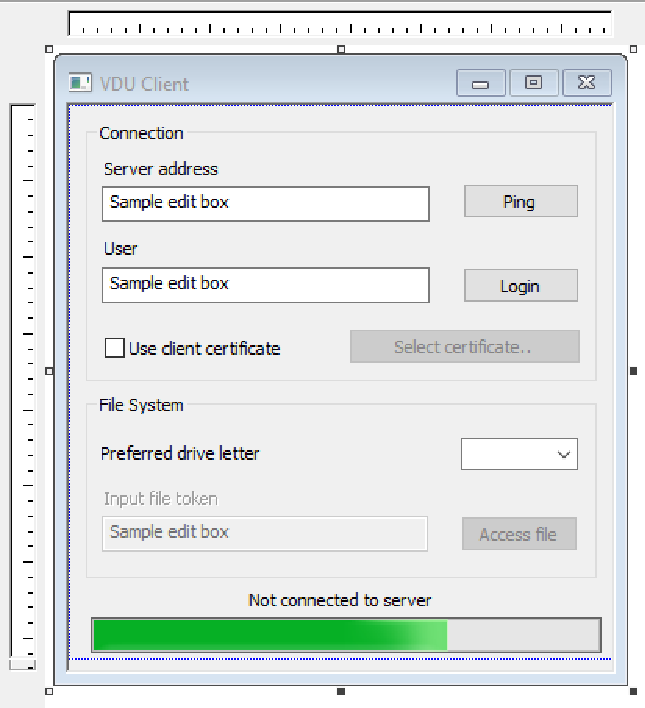
\includegraphics[]{obrazky-figures/resourceeditorui.pdf}
	\caption{The VDU Client dialog window user interface, as designed in Visual Studio dialog editor.}
	\label{dialogeditorui}
\end{figure}
Each designed window serves as a template for programatically created windows of the same type, and has a unique identifier - \textit{name}. When creating a window, a template can be specified to guide the design of this window. As shown in Listing \ref{cdialogex}, the \lstinline{Create} function of \lstinline{CDialogEx} is uses the designed window template specified as the first parameter.
\begin{lstlisting}[caption={Creating the extended dialog window of VDU Client}, label=cdialogex]
CVDUClientDlg* pDlg = new CVDUClientDlg();
pDlg->Create(IDD_VDUCLIENT_DIALOG, AfxGetMainWnd());
\end{lstlisting}
\subsubsection{Event handlers}
In Windows, whenever a window is interacted with it receives a message, which can be handled and responded to. MFC provides a way to implement a function, which gets called when a specific message is received - an \textit{event handler}. For each child window of the dialog, including itself, I implemented one or more event handlers to assure functionality of the interface. An example of an event handler, along with it's mapping to a message and impelementation is displayed in Listing \ref{messagemapping}. 
\newpage
\begin{lstlisting}[caption={Example of implemented and mapped click event handler}, label=messagemapping]
//Message mapping for dialog
BEGIN_MESSAGE_MAP(CVDUClientDlg, CDialogEx)
	ON_BN_CLICKED(IDC_BUTTON_PING, &CVDUClientDlg::OnBnClickedPing)
END_MESSAGE_MAP()

void CVDUClientDlg::OnBnClickedPing()
{
	TryPing();
	...
}
\end{lstlisting}

\subsubsection{Tray}
The core of interacting with the Windows tray area, and creating a tray icon, is the \lstinline{Shell_NotifyIcon}\footnote{\url{https://docs.microsoft.com/en-us/windows/win32/api/shellapi/nf-shellapi-shell_notifyiconw}} function of the Windows API. The information about tray icon is stored in \lstinline{m_trayData} inside \lstinline{CVDUClientDlg}. This data is modified and sent to the function whenever an operation with the tray icon is required. I divided interactions with the tray area into four parts:
\begin{itemize}
    \item \textit{Create } - \lstinline{Shell_NotifyIcon(NIM_ADD, &m_trayData);}
    \item \textit{Update tip} - \lstinline{Shell_NotifyIcon(NIM_ADD, &m_trayData);}
    \item \textit{Send notification} - \lstinline{Shell_NotifyIcon(NIM_ADD, &m_trayData);}
\end{itemize}

To make it seem like the window gets hidden to tray, I override the system command \lstinline{SC_CLOSE} to minimize and hide the window instead using the . \ref{sysclose}

\begin{lstlisting}[caption={Overriding system close command to hide the dialog window}, label=sysclose]
void CVDUClientDlg::OnSysCommand(UINT nID, LPARAM lParam)
{
	if ((nID & 0xFFF0) == SC_CLOSE)
	{
		ShowWindow(SW_MINIMIZE);
		ShowWindow(SW_HIDE);
		return;
	}

	CDialogEx::OnSysCommand(nID, lParam);
}
\end{lstlisting}

\subsubsection{Message box}

\subsection{Windows environment}
This subsection covers features, which tie closely to the Windows environment, such as the use of the tray area and the automatic start up of the application when the Windows user logs in.

\subsubsection{}

%=============================================================================================================================
\chapter{Testing}
\label{ch_testing}
%=============================================================================================================================
Application testing is a key development process used to assert and verify the application's correct functionality and the presence of its required properties. In the VDU Client case, the requirement is to enable the application to be tested using automated tests. Automating the testing of a Windows GUI\footnote{Graphical User Interface} application that appears to be entirely controlled by the user's input can prove to be challenging at first. With good knowledge of the Windows API, visualizations from analysis in chapter \ref{ch_analysis}, and a scripting language, I was able to simulate a VDU server and create an expandable testing script that made implementing and running automated tests easier and better scalable.

\section{VDU server simulation}
Due to the network connectivity requirements of the client-server type of applications, it is difficult to provably test the functionality and properties of the client without the presence of the server. Additionally, the risk of flooding the production server due to automated testing might lower the quality of service for real users. This is the motivation behind creating a \textit{simulated VDU server}, which would only be present locally and respond to the client's requests. This approach comes with several advantages:
\begin{itemize}
    \item \textit{Independence} - Even if the VDU server stops working, testing can continue
    \item \textit{Interface stability} - A sudden change in the interface of the VDU server will not affect the application
    \item \textit{Flexibility} - Application can be modified and properly tested over time to comply with any changes on the server
    \item \textit{Transfer speed} - Transferring of files is limited only by the speed of the local network
\end{itemize}

\subsection{Specifications and analysis}
In this section, the formal VDU server API specifications, analyzed in chapter \ref{ch_analysis}, are an important point of reference. As this specification clearly states, the VDU server communicates over the HTTP protocol in TLS\footnote{Transport Layer Security}/HTTP channel and provides a REST API interface to interact with. Knowing this, the VDU server can be simplified down to a program that:
\begin{itemize}
    \item \textit{Hosts an HTTP server with a secure TLS channel}
    \item \textit{Is able to read and modify files}
\end{itemize}
Alternatively, in order for the simulated server to behave just like a real VDU server, it needs to simulate every endpoint of the real VDU server. The exact implementation of either server is not relevant for this purpose.

\subsection{Design}
Given the simplistic nature of the program requirements, in order to save time while sacrificing little to no functionality, I have decided to create the simulated VDU server using Python\footnote{\url{https://www.python.org/}}.

\subsubsection{Python}
Python is an interpreted, simple, easy to learn programming language with emphasis on its syntax's readability. It is considered a high-level language, allows for object-oriented programming and dynamic typing. A program written in the Python programming language is referred to as a Python script since it is interpreted using the Python interpreter, which comes equipped with feature-rich default libraries that are completely able to cover the requirements for a simulated VDU server, as described by \cite{PythonWhatis}. These facts make Python a great programming language choice for the implementation of the server.
\subsubsection{Simulating endpoints}
 While knowing the exact implementation of the server would make the simulation more precise, it was unknown for the purposes of this thesis. Thanks to the properly detailed specification and description of each endpoint, simulating every single endpoint was still possible.
 
\subsection{Design}
 
\subsection{Implementation}
 
\subsection{Supporting HTTPS/TLS}
\todo{Should I include how TLS works in the theory part? Certificates, CAs, asymmetric encryption, and stuff seems a bit too much maybe?}
Due to the fact that the real server uses HTTPS protocol to communicate with the client, the simulated server should be supporting the secure channel connection as well. In order to start the Python HTTP server in a way, which allows for HTTPS connections with the possibility of accepting client certificates, it required three important parts:
\begin{itemize}
    \item \textit{Certificate authority} - used to generate certificates
    \item \textit{Server certificate} - contains the server's public key
    \item \textit{Server key file} - contains the server's private key
\end{itemize}
It would be wasteful to acquire certificates from legitimate authorities, as the simulated VDU server will not be used for any purposes other than testing. Instead, I decided to solve this problem by creating a testing certificate authority (CA) using OpenSSL\footnote{\url{https://www.openssl.org/}}. Upon creating my own testing CA, I used OpenSSL again to issue a testing certificate for the simulated VDU server. This operation generated both a public and a private key. 

With CA and the server certificate generated, I wrapped the Python HTTP server's socket to use them and not require a client certificate from incoming connections. This operation allows the VDU application to successfully connect to the simulated server, assuming the application will ignore the invalidity of the CA. How I modified the application to support this is described in section \ref{ignorecerts}.
This subsection was created and implemented with the help of \cite{SSLCertTut}.
\section{Modifying the application}
By default, the application can only be controlled by the user using its user interface. This fact makes it difficult to test the application in an automated manner - issuing commands to the GUI\footnote{Graphical User Interface} is not practical. A much better solution for this problem is to create a special mode in which the application is able to be launched - the \textit{testing mode}.

\subsection{Testing mode}

\subsection{Ignoring untrusted certificates}
\label{ignorecerts}

\section{Automated testing script}

\subsection{C}

%=============================================================================================================================
\chapter{Conclusion}
\label{ch_conclusion}
\todo{Evaluation of progress etc.}

The result application was released, and I published the source code as open-source on GitHub\footnote{\url{https://github.com/}}.

%=============================================================================================================================

  \else
    \input{xferan00-vdu-windows-01-kapitoly-chapters}
  \fi
  
  % Kompilace po částech (viz výše, nutno odkomentovat)
  % Compilation piecewise (see above, it is necessary to uncomment it)
  %\subfile{xferan00-vdu-windows-01-uvod-introduction}
  % ...
  %\subfile{chapters/xferan00-vdu-windows-05-conclusion}


  % Pouzita literatura / Bibliography
  % ----------------------------------------------
\ifslovak
  \makeatletter
  \def\@openbib@code{\addcontentsline{toc}{chapter}{Literatúra}}
  \makeatother
  \bibliographystyle{bib-styles/Pysny/skplain}
\else
  \ifczech
    \makeatletter
    \def\@openbib@code{\addcontentsline{toc}{chapter}{Literatura}}
    \makeatother
    \bibliographystyle{bib-styles/Pysny/czplain}
  \else 
    \makeatletter
    \def\@openbib@code{\addcontentsline{toc}{chapter}{Bibliography}}
    \makeatother
    \bibliographystyle{bib-styles/Pysny/enplain}
  %  \bibliographystyle{alpha}
  \fi
\fi
  \begin{flushleft}
  \bibliography{xferan00-vdu-windows-20-literatura-bibliography}
  \end{flushleft}

  % vynechani stranky v oboustrannem rezimu
  % Skip the page in the two-sided mode
  \iftwoside
    \cleardoublepage
  \fi

  % Prilohy / Appendices
  % ---------------------------------------------
  \appendix
\ifczech
  \renewcommand{\appendixpagename}{Přílohy}
  \renewcommand{\appendixtocname}{Přílohy}
  \renewcommand{\appendixname}{Příloha}
\fi
\ifslovak
  \renewcommand{\appendixpagename}{Prílohy}
  \renewcommand{\appendixtocname}{Prílohy}
  \renewcommand{\appendixname}{Príloha}
\fi
%  \appendixpage

% vynechani stranky v oboustrannem rezimu
% Skip the page in the two-sided mode
%\iftwoside
%  \cleardoublepage
%\fi
  
\ifslovak
%  \section*{Zoznam príloh}
%  \addcontentsline{toc}{section}{Zoznam príloh}
\else
  \ifczech
%    \section*{Seznam příloh}
%    \addcontentsline{toc}{section}{Seznam příloh}
  \else
%    \section*{List of Appendices}
%    \addcontentsline{toc}{section}{List of Appendices}
  \fi
\fi
  \startcontents[chapters]
  \setlength{\parskip}{0pt} 
  % seznam příloh / list of appendices
  % \printcontents[chapters]{l}{0}{\setcounter{tocdepth}{2}}
  
  \ifODSAZ
    \setlength{\parskip}{0.5\bigskipamount}
  \else
    \setlength{\parskip}{0pt}
  \fi
  
  % vynechani stranky v oboustrannem rezimu
  \iftwoside
    \cleardoublepage
  \fi
  
  % Přílohy / Appendices
  \ifenglish
    % This file should be replaced with your file with an appendices (headings below are examples only)

% Placing of table of contents of the memory media here should be consulted with a supervisor
\chapter{Contents of the included storage media}

%\chapter{Manual}

%\chapter{Configuration file}

%\chapter{Scheme of RelaxNG configuration file}

%\chapter{Poster}

  \else
    \input{xferan00-vdu-windows-30-prilohy-appendices}
  \fi
  
  % Kompilace po částech (viz výše, nutno odkomentovat)
  % Compilation piecewise (see above, it is necessary to uncomment it)
  %\subfile{xferan00-vdu-windows-30-prilohy-appendices}
  
\end{document}
